\documentclass[mathserif]{beamer}

\usepackage{nips15}

%-----------------------------------------------------------------------
\usepackage{pdfpages}
\usepackage{array}
\usepackage{booktabs}
\usepackage[skins,breakable]{tcolorbox}
\usepackage{minibox}
\usepackage{mathtools}

\newcommand{\todo}[1]{{\scriptsize\color{yellow}\textsc{[Todo]}}}

\newcommand{\qcite}[1]{{\scriptsize\color{col2}[#1]}}

\newcommand{\qboxa}[1]{%
\begin{tcolorbox}[enhanced jigsaw,size=tight,hbox,boxsep=4pt,boxrule=1pt,coltext=textcolor,colframe=col1,opacityback=0,opacityframe=1]
\strut #1
\end{tcolorbox}%
}

\newcommand{\qboxb}[1]{%
\begin{tcolorbox}[enhanced jigsaw,size=tight,hbox,boxsep=4pt,boxrule=1pt,coltext=textcolor,colframe=col2,opacityback=0,opacityframe=1]
\strut #1
\end{tcolorbox}%
}

\newcommand{\qtheorem}[2]{%
\begin{tcolorbox}[enhanced jigsaw,size=tight,boxsep=7pt,boxrule=0.7pt,coltext=textcolor,colframe=col2,colback=col1,opacityback=0,opacityframe=1]
\begin{minipage}{\textwidth}
{\color{col2}\strut Theorem #1}\\[0.7em]
#2
\end{minipage}
\end{tcolorbox}%
}

\newcommand{\qlemma}[1]{%
\begin{tcolorbox}[enhanced jigsaw,size=tight,boxsep=7pt,boxrule=0.7pt,coltext=textcolor,colframe=col2,colback=col1,opacityback=0,opacityframe=1]
\begin{minipage}{\textwidth}
{\color{col2}\strut Lemma}\\[0.7em]
#1
\end{minipage}
\end{tcolorbox}%
}
%-----------------------------------------------------------------------

\title[Sampling from Probabilistic Submodular Models]
{Sampling from Probabilistic Submodular Models}

\author[Alkis Gotovos]{}

\begin{document}

\setbeamertemplate{background canvas}{}
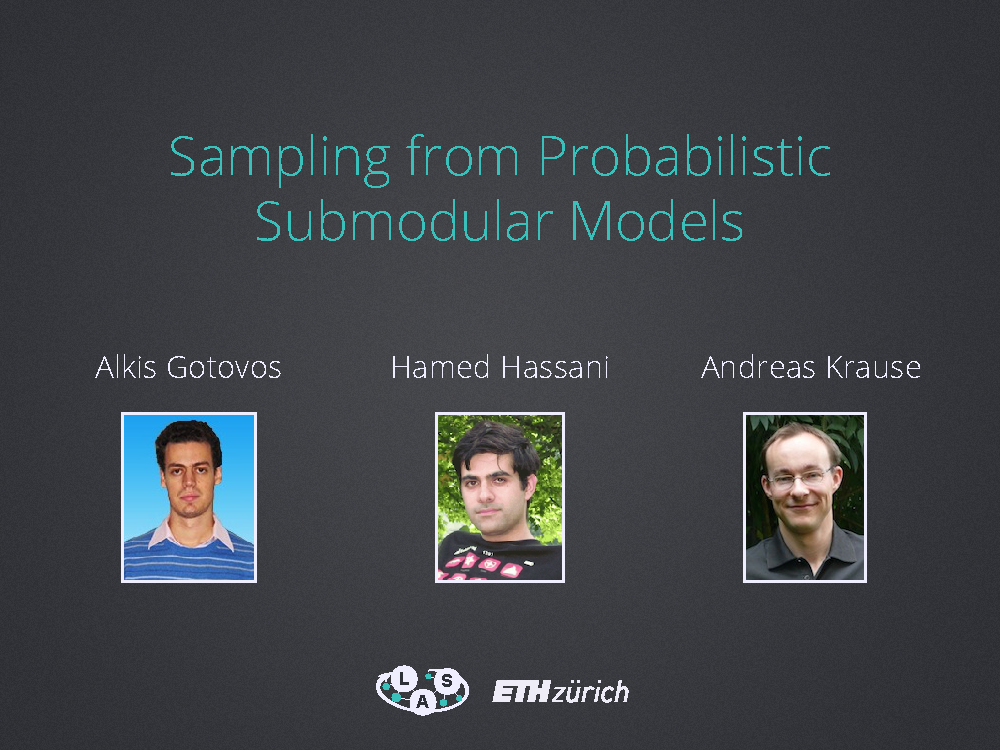
\includepdf[pages={1}]{title.pdf}
\setbeamertemplate{background canvas}{
\includegraphics[width=\paperwidth]{figures/bg.png}}

\begin{frame}{Image Collection Summarization}
\vspace{0.5em}
\centering
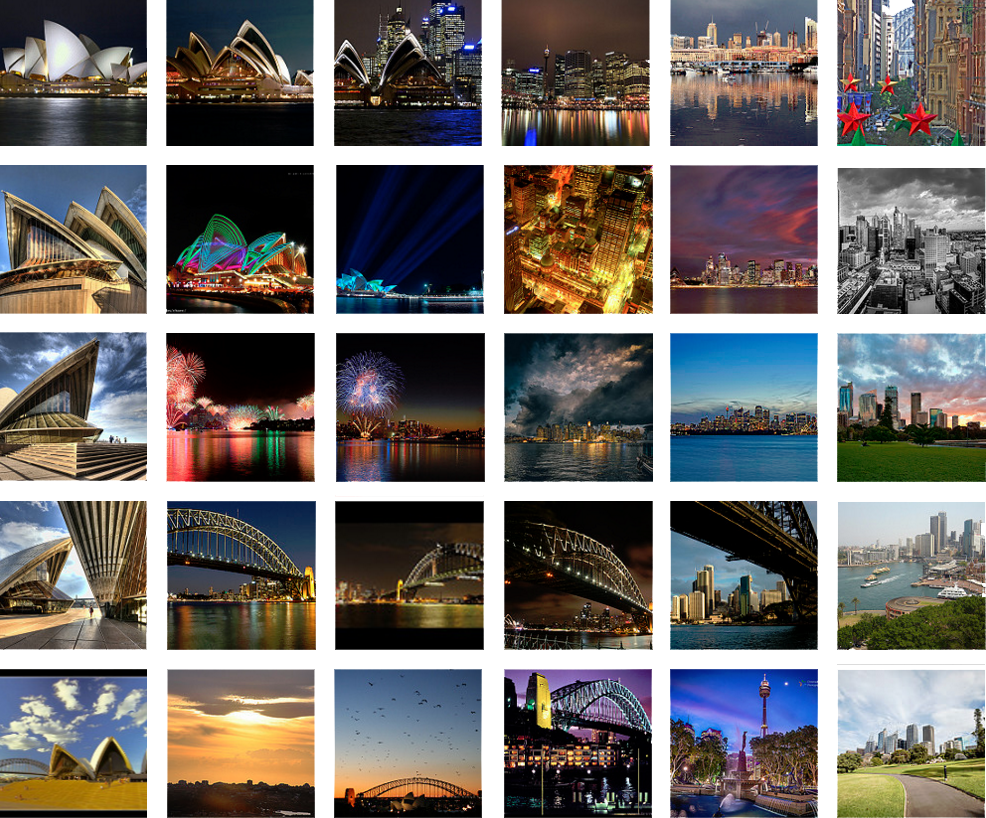
\includegraphics[width=3.6in]{figures/flickr_probs_0.png}
\end{frame}

\begin{frame}{Submodularity}
\vspace{0.5em}
\begin{itemize}
\item<1-> Facility location objective \qcite{Lin and Bilmes, '12} \qcite{Tschiatschek et al., '14}
\vspace{0.5em}
\item<2-> Encourage coverage and diversity of the summary
\vspace{0.5em}
\item<3-> Set of all images $V$
\vspace{0.5em}
\item<4-> For any summary $S \subseteq V\ \ \longrightarrow\ \ F(S) \in \mathbb{R}$
\end{itemize}

\vspace{0.5em}
\centering
\alt<1-5>{
\uncover<5>{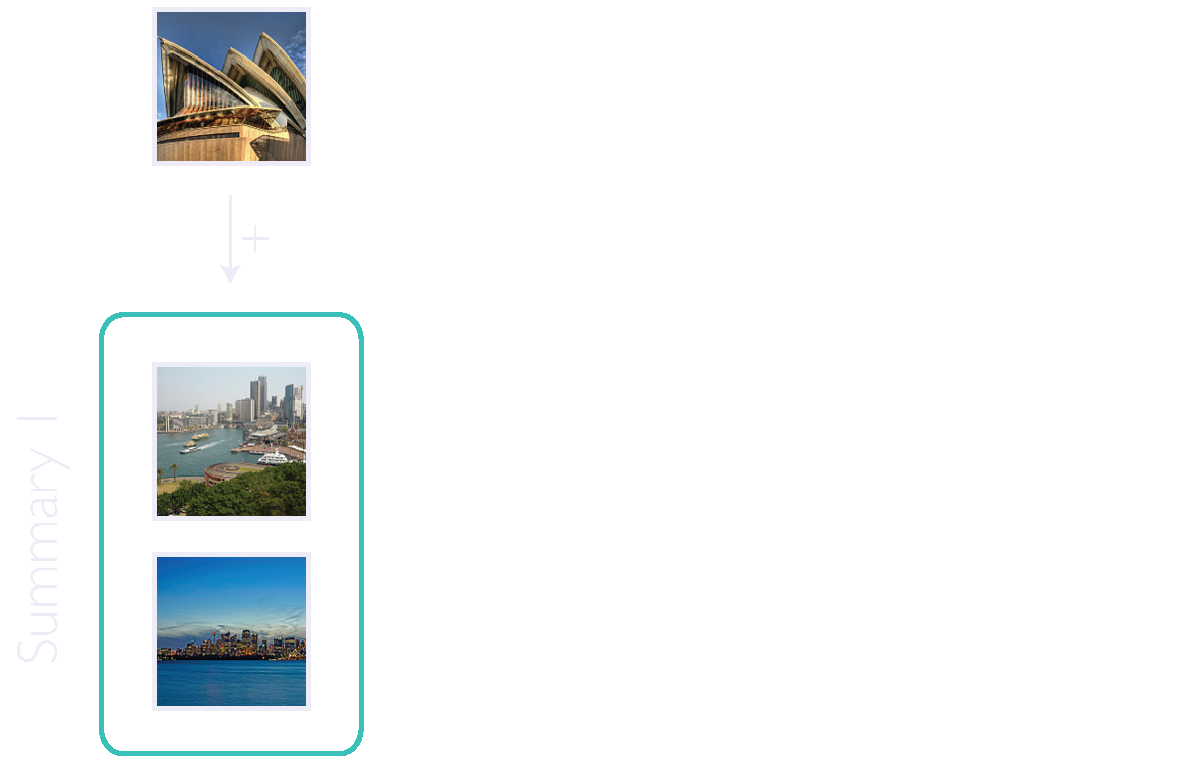
\includegraphics[width=2.75in]{figures/submod_1.pdf}}%
}{}%
\only<6>{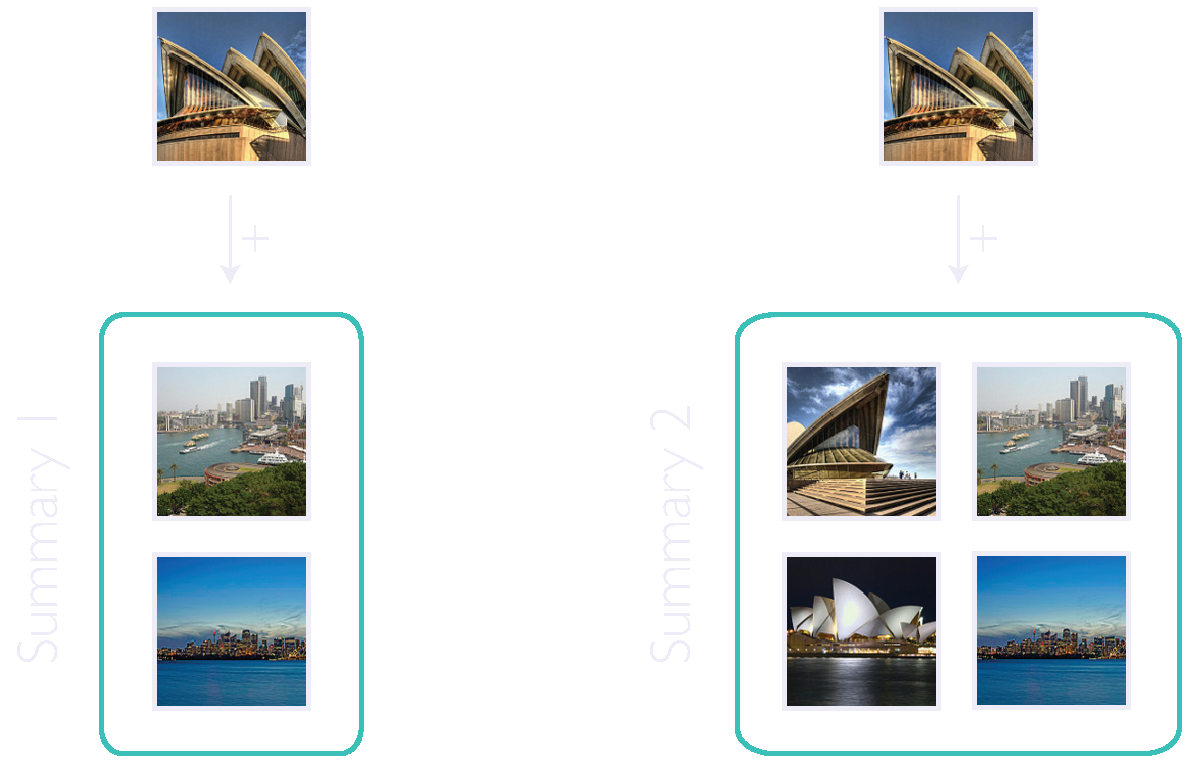
\includegraphics[width=2.75in]{figures/submod_2.pdf}}%
\only<7>{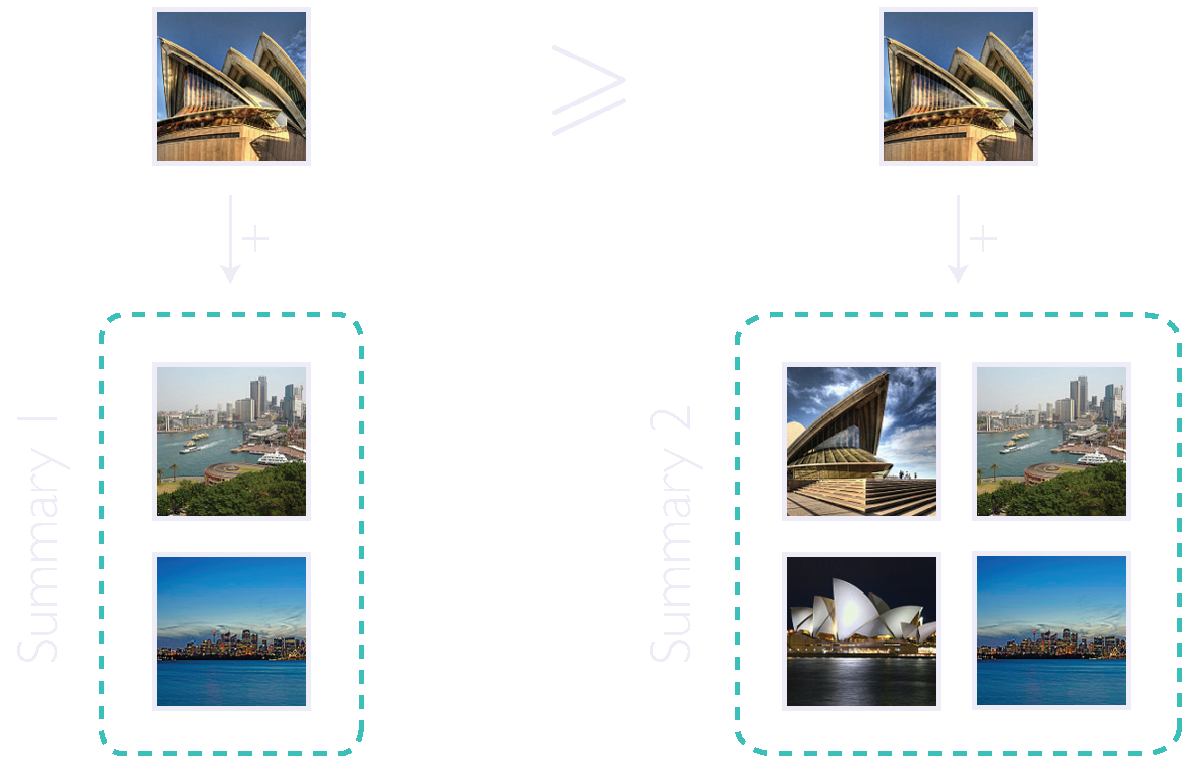
\includegraphics[width=2.75in]{figures/submod_3.pdf}}
\end{frame}

\begin{frame}{Submodularity}
\vspace{0.5em}
\uncover<1->{
\begin{tabular}{c*{2}{@{\hspace{3em}}c}}
$F$ is submodular & $\Longleftrightarrow$ & $-F$ is supermodular\\[0.5em]
$\downarrow$ & & $\downarrow$\\[0.5em]
\qboxa{coverage / diversity} & & \qboxb{smoothness / cooperation}
\end{tabular}
}

\vspace{2em}
\begin{itemize}
\item<2-> Submodular optimization is well-studied
\vspace{1em}
\item<3-> Little existing work on probabilistic models
\end{itemize}
\end{frame}

\begin{frame}{Sampling Summaries}
\vspace{1em}
\centering
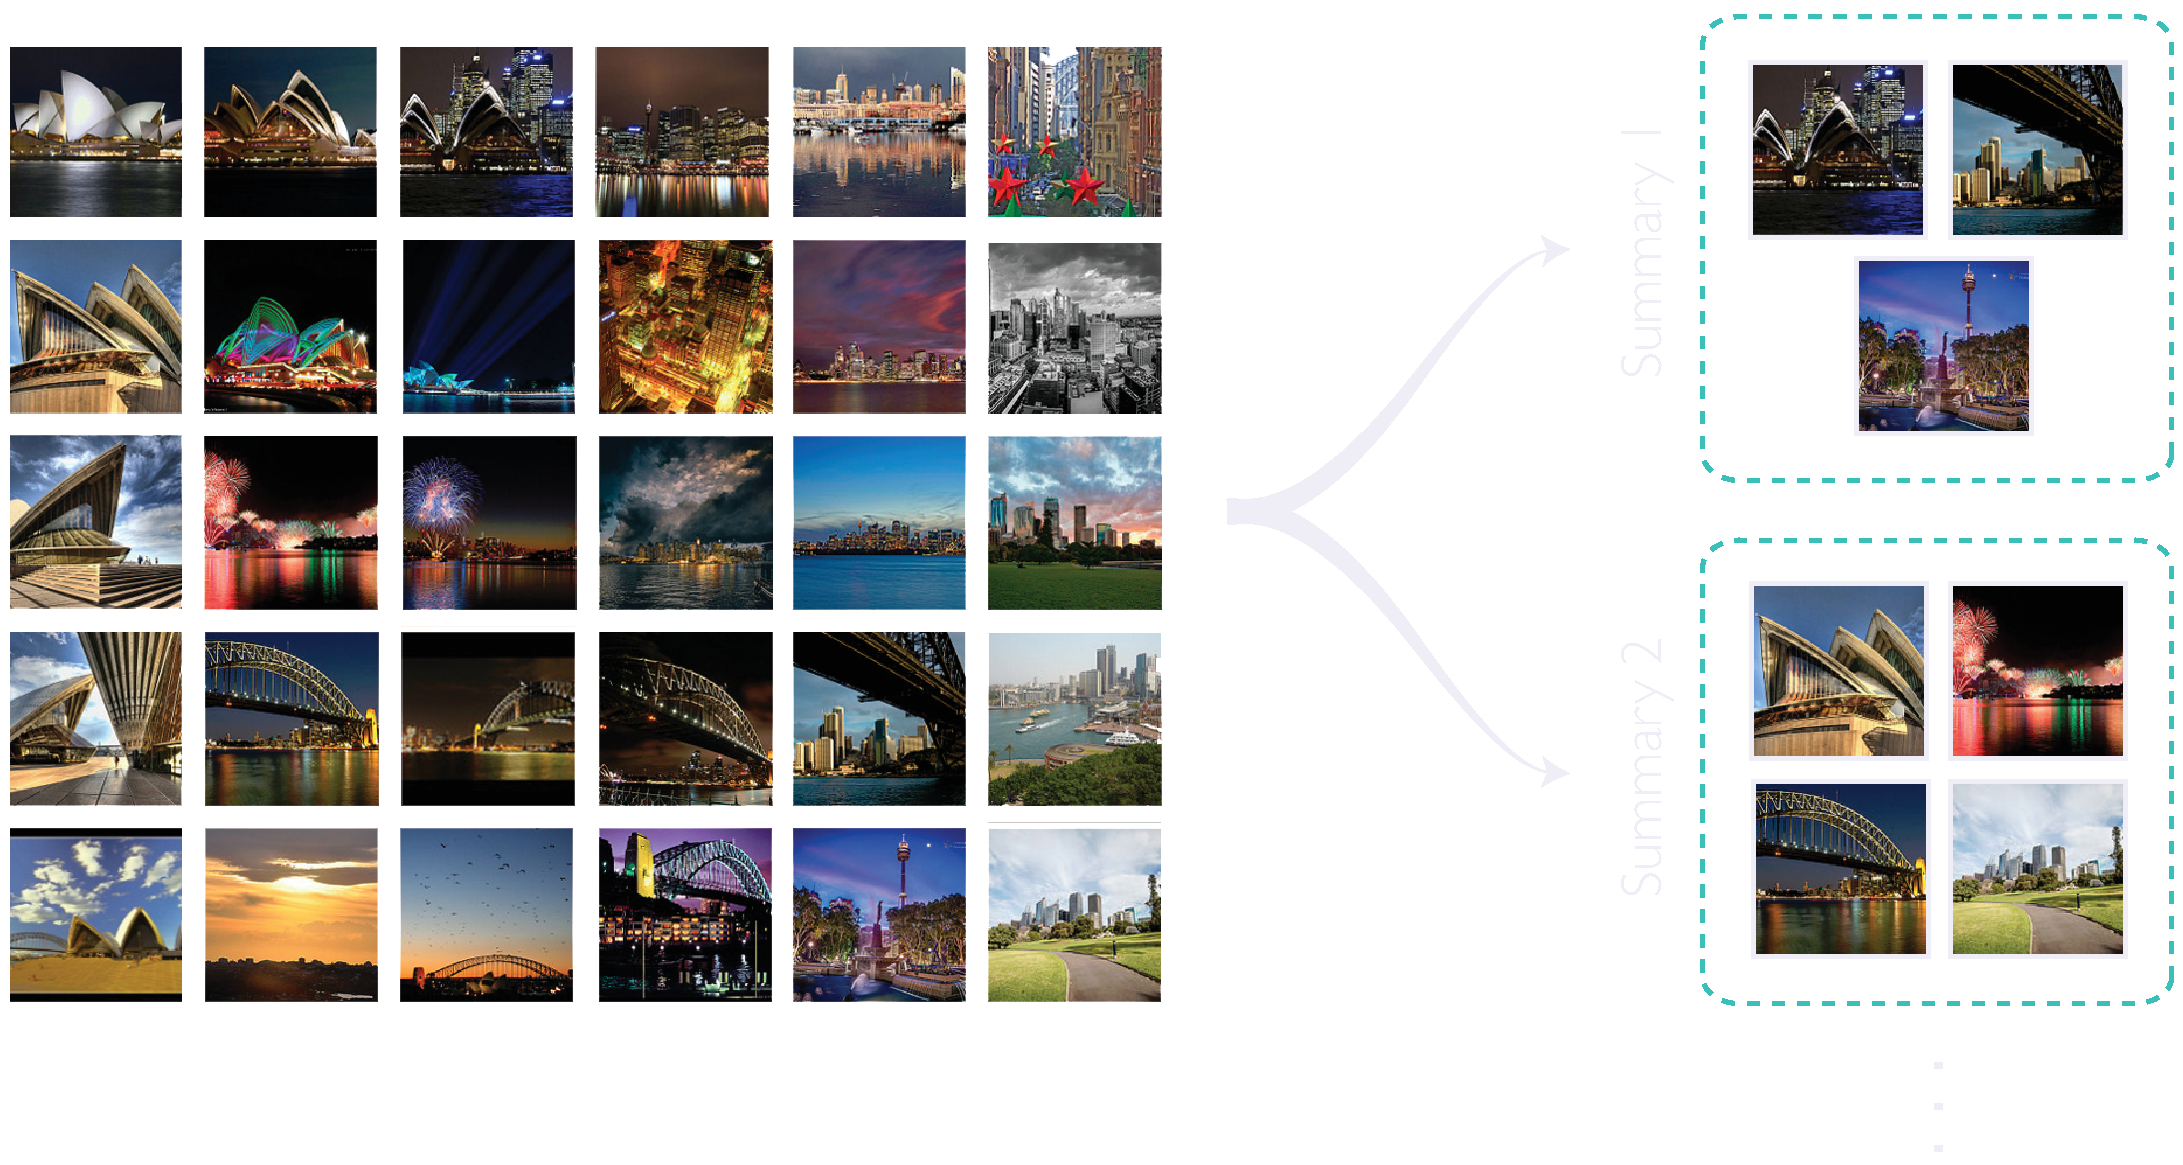
\includegraphics[width=4.2in]{figures/flickr_summaries.pdf}
\end{frame}

\begin{frame}{Foreground / Background Segmentation}
\vspace{0.5em}
\begin{columns}[c]
\column{0.5\textwidth}
\centering
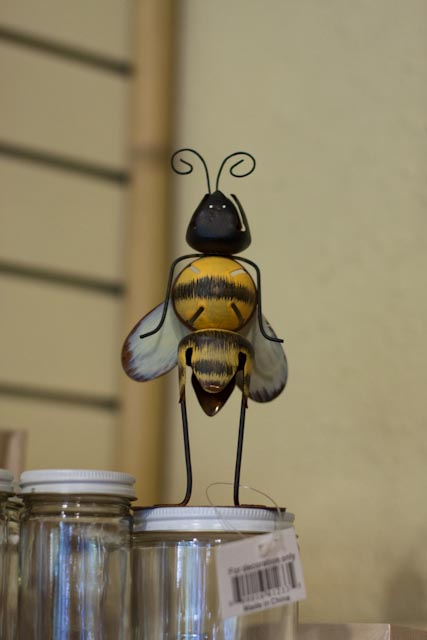
\includegraphics[width=1.8in]{figures/bee.jpg}

\column{0.5\textwidth}
\centering
\only<2>{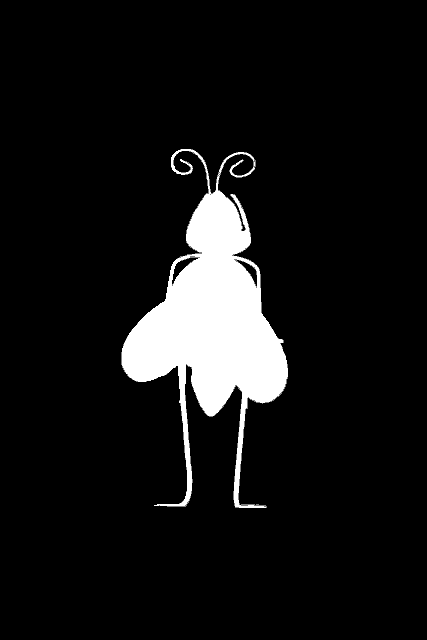
\includegraphics[width=1.8in]{figures/bee_truth.png}}%
\only<3>{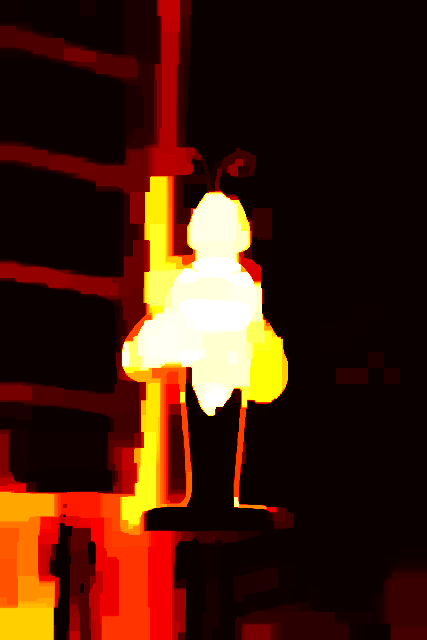
\includegraphics[width=1.8in]{figures/bee_dr1.png}}%
\only<4-6>{
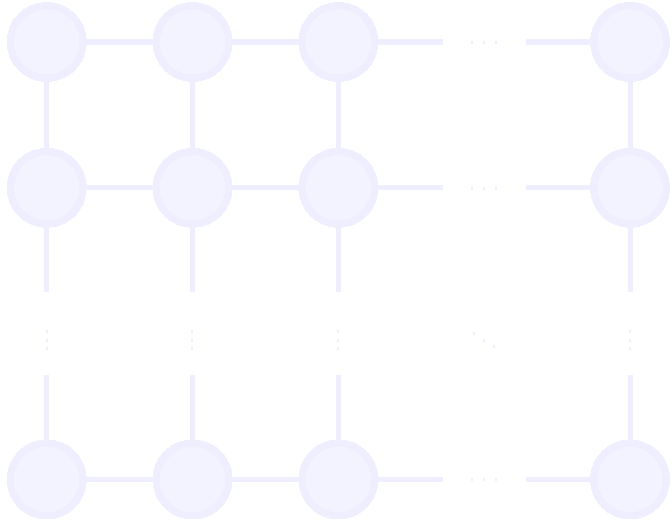
\includegraphics[width=1.5in]{figures/grid.pdf}

\vspace{0.5em}
\begin{itemize}
\item<5-> Set of all pixels $V$
\vspace{1em}
\item<6-> For $S \subseteq V$ of foreground pixels,
\begin{align*}
p(S) \propto \exp\left(\sum_{v \sim w} F_{v, w}(S)\right)
\end{align*}
\end{itemize}
}
\end{columns}
\end{frame}

\begin{frame}{Higher-order Models}
\vspace{0.5em}
\begin{columns}[c]
\column{0.5\textwidth}
\centering
\only<1-2,6>{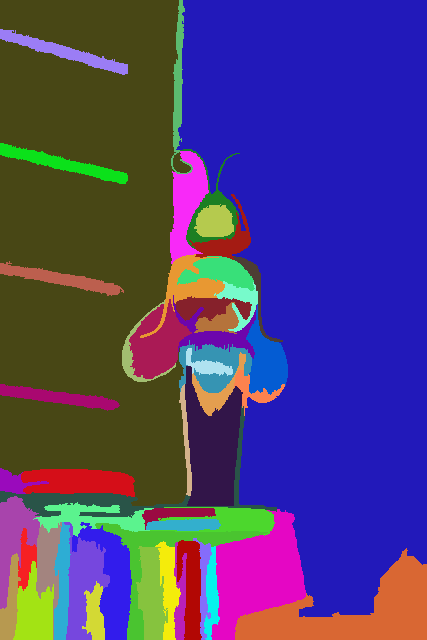
\includegraphics[width=1.8in]{figures/bee_superpixels.png}}%
\only<3-5>{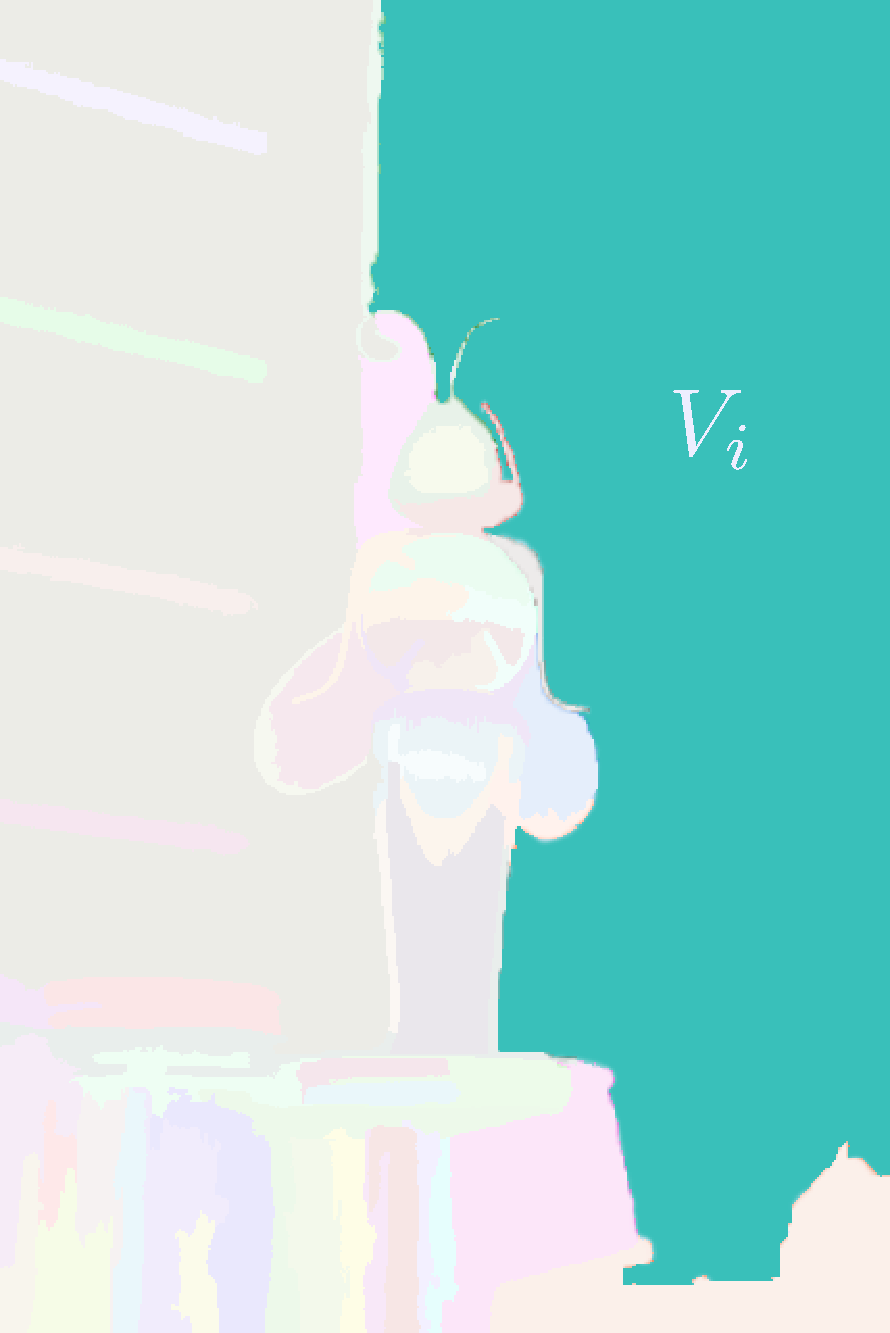
\includegraphics[width=1.8in]{figures/bee_superpixels_hl_v1.pdf}}

\vspace{0.5em}
\centering
{\small Superpixel potentials} \qcite{Kohli et al., '08}
\column{0.5\textwidth}
\uncover<2->{
$V = V_1 \cup V_2 \cup \cdots \cup V_L$
}

\uncover<4->{
\vspace{1em}
$F_i(S) = \phi\left(|S \cap V_i|\right)$
}

\uncover<5->{
\vspace{1.3em}
\hspace{-1.5em}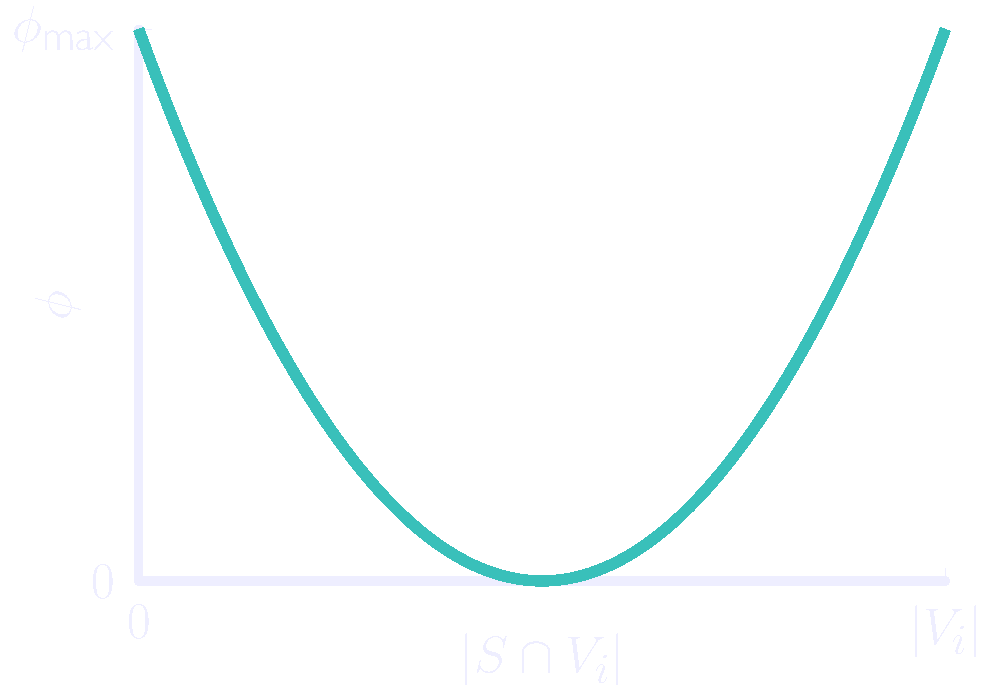
\includegraphics[width=2.1in]{figures/convex_over_modular.pdf}
}

\uncover<6->{
\vspace{1em}
$p(S) \propto \exp\left(\displaystyle\sum_{i=1}^L F_i(S)\right)$
}
\end{columns}
\end{frame}

\begin{frame}{Higher-order Models \qcite{Djolonga and Krause, '15}}
\vspace{0.5em}
\begin{columns}[c]
\column{0.5\textwidth}
\centering
\strut Pairwise

\vspace{0.3em}
\centering
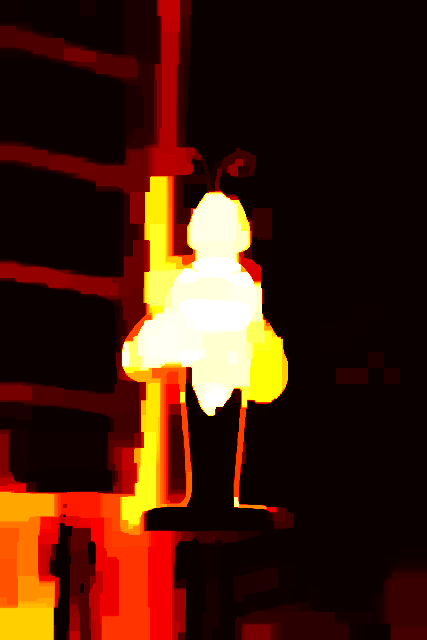
\includegraphics[width=1.8in]{figures/bee_dr1.png}

\column{0.5\textwidth}
\centering
\strut Higher-order

\vspace{0.3em}
\centering
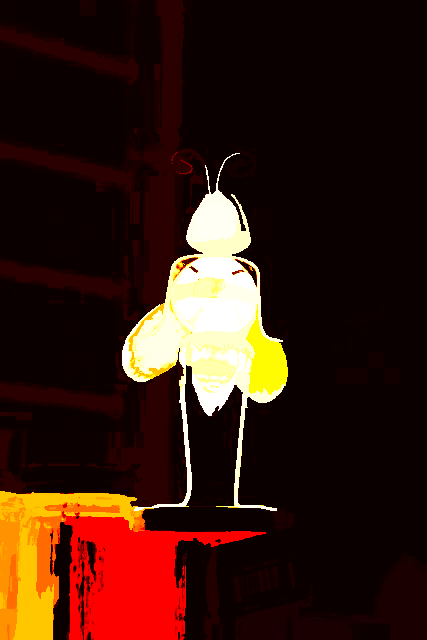
\includegraphics[width=1.8in]{figures/bee_marginals.png}
\end{columns}
\end{frame}

\begin{frame}{Probabilistic Submodular Models}
\vspace{0.5em}
\centering
\only<1>{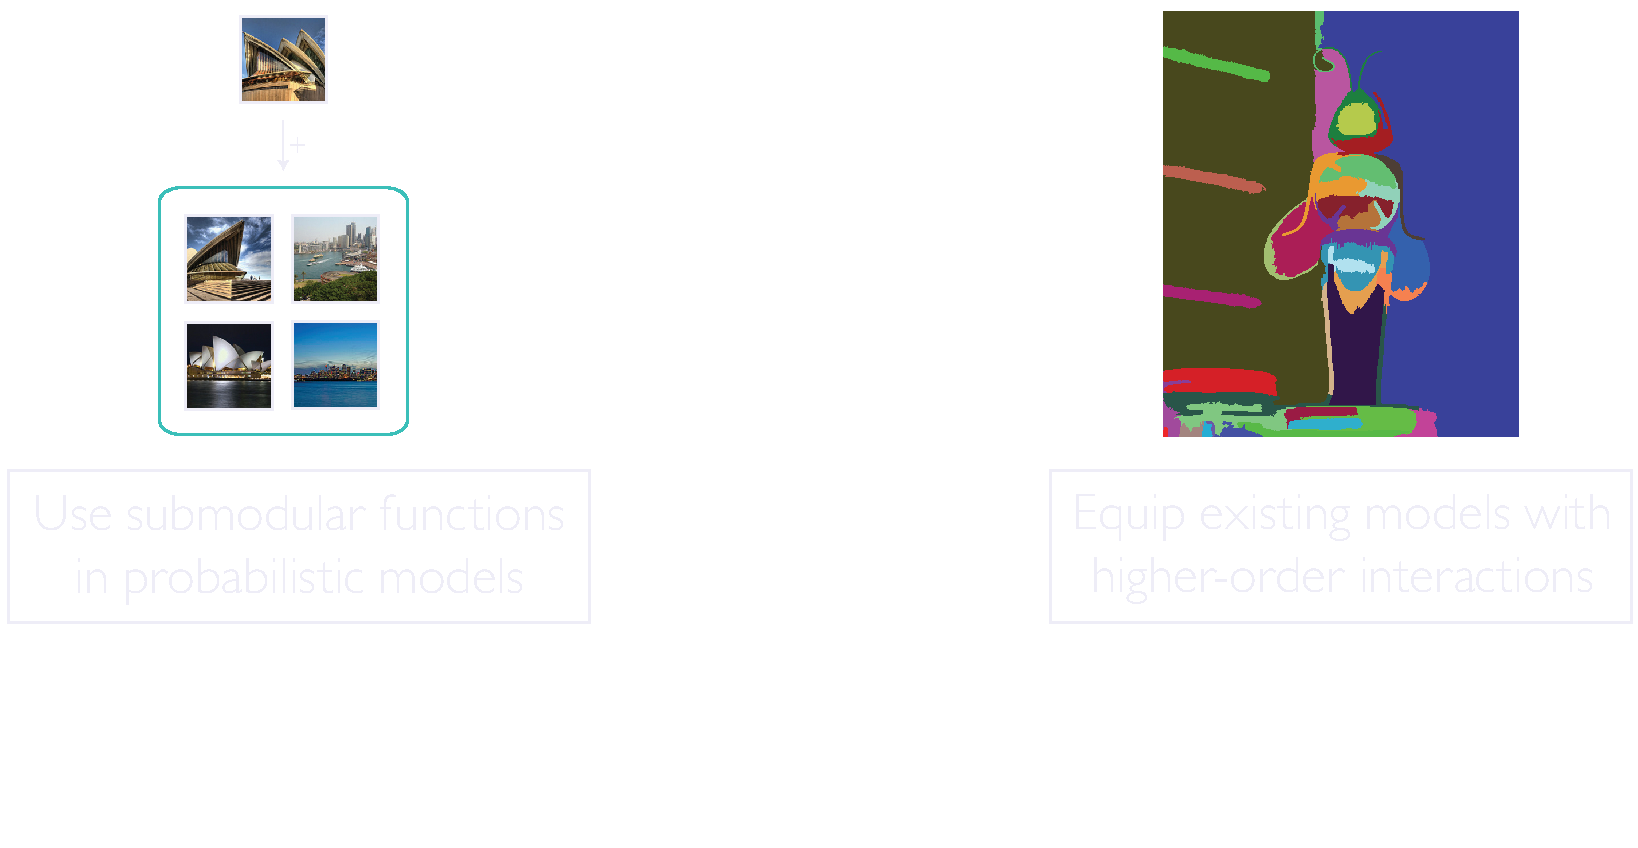
\includegraphics[width=4.2in]{figures/psm_0.pdf}}%
\only<2->{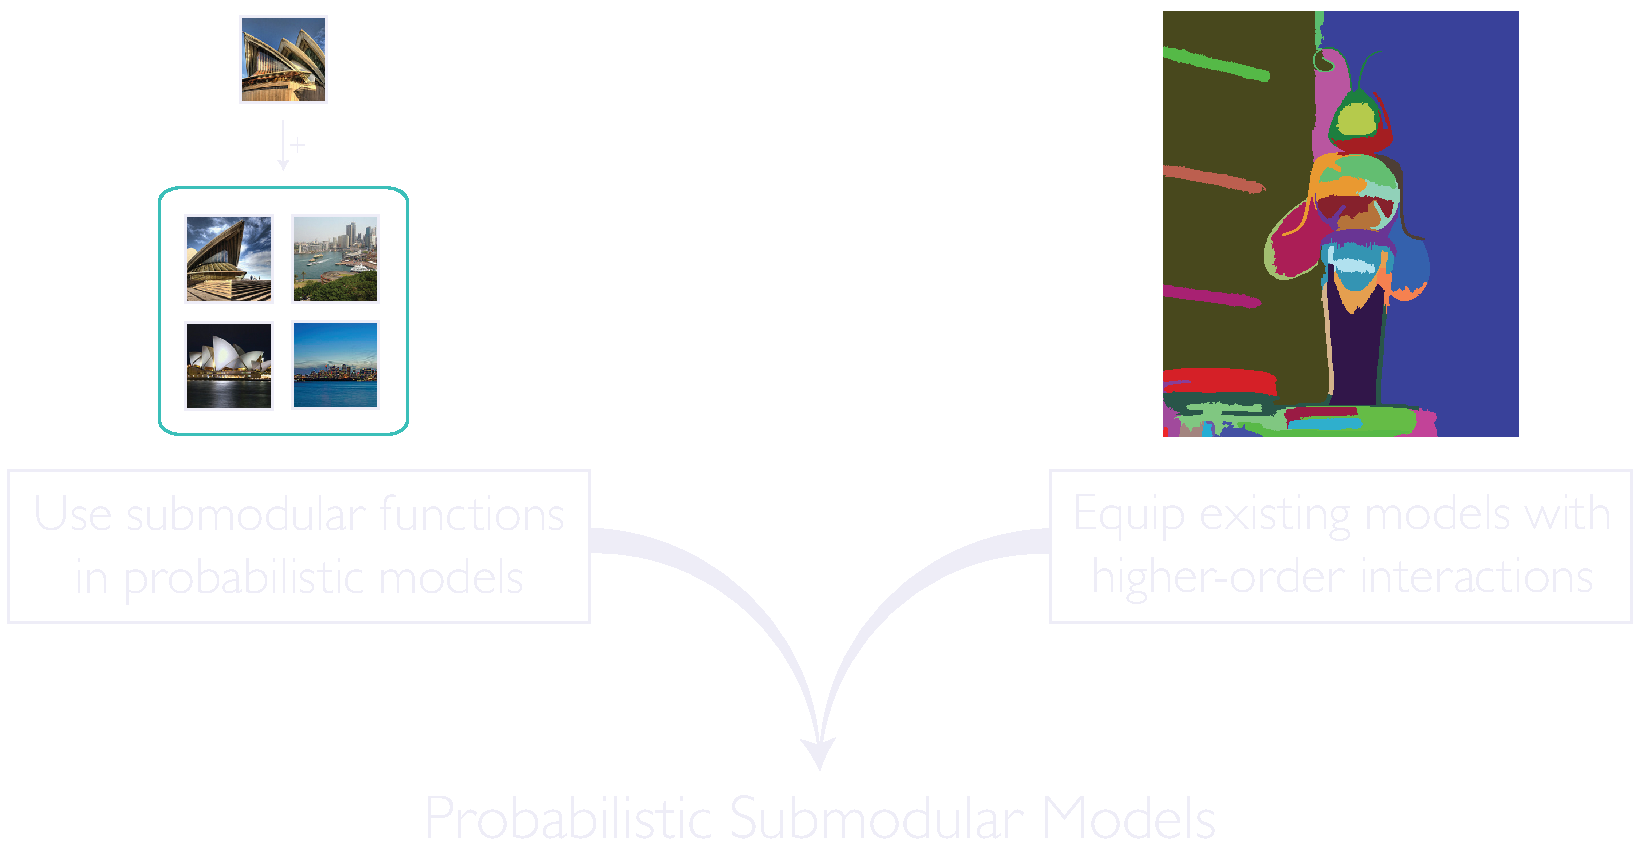
\includegraphics[width=4.2in]{figures/psm_1.pdf}}

\uncover<3->{
\vspace{0.5em}
\qboxa{$p(S) = \displaystyle\frac{1}{Z} \exp(F(S))$} $F : 2^V \to \mathbb{R}$ is a submodular or supermodular function
}
\end{frame}

\begin{frame}{Probabilistic Submodular Models}
\vspace{1em}
\renewcommand{\arraystretch}{1.4}
\begin{tabular}{>{\arraybackslash}p{0.47\textwidth}>{\arraybackslash}p{0.45\textwidth}}
\centering\arraybackslash {\large PSMs} & \centering\arraybackslash {\large \minibox{Markov Random Fields\\[0.2em]}}\\ \toprule

\begin{minipage}[t]{\textwidth}
\begin{itemize}
\item<2-> Ground set $V$ with $|V| = n$
\end{itemize}
\end{minipage}
&
\begin{minipage}[t]{\textwidth}
\begin{itemize}
\item<5-> Binary random vector

\vspace{0.7em}
\hspace{1em}$X = (X_1, \ldots, X_n)$

\vspace{0.5em}
\end{itemize}
\end{minipage}\\

\begin{minipage}[t]{\textwidth}
\begin{itemize}
\item<3->Sub- or supermodular function

\vspace{0.7em}
\hspace{1em}$F : 2^V \to \mathbb{R}$
\end{itemize}
\end{minipage}
&
\begin{minipage}[t]{\textwidth}
\begin{itemize}
\item<6-> Set of factors

\vspace{0.7em}
\hspace{1em}$\phi_i : \{0,1\}^{\mathcal{C}_i} \to \mathbb{R}$

\vspace{0.7em}
\end{itemize}
\end{minipage}\\

\begin{minipage}[t]{\textwidth}
\begin{itemize}
\item<4-> Distribution over subsets

\vspace{0.7em}
\hspace{1em}$p(S) \propto \exp(F(S))$
\end{itemize}
\end{minipage}
&
\begin{minipage}[t]{\textwidth}
\begin{itemize}
\item<7-> Distribution over binary vectors

\vspace{0.45em}
$p(X) \propto \exp\Big(\sum_i \phi_i\left(X_{\mathcal{C}_i}\right)\Big)$
\end{itemize}

\vspace{0.1em}
\end{minipage}\\ \midrule
\end{tabular}

\uncover<8>{
\vspace{0.15em}
\centering
\qboxa{Model order: $\max_i |\mathcal{C}_i|$}}
\end{frame}

\begin{frame}{Landscape of Models}
\vspace{0.5em}
\centering
\only<1>{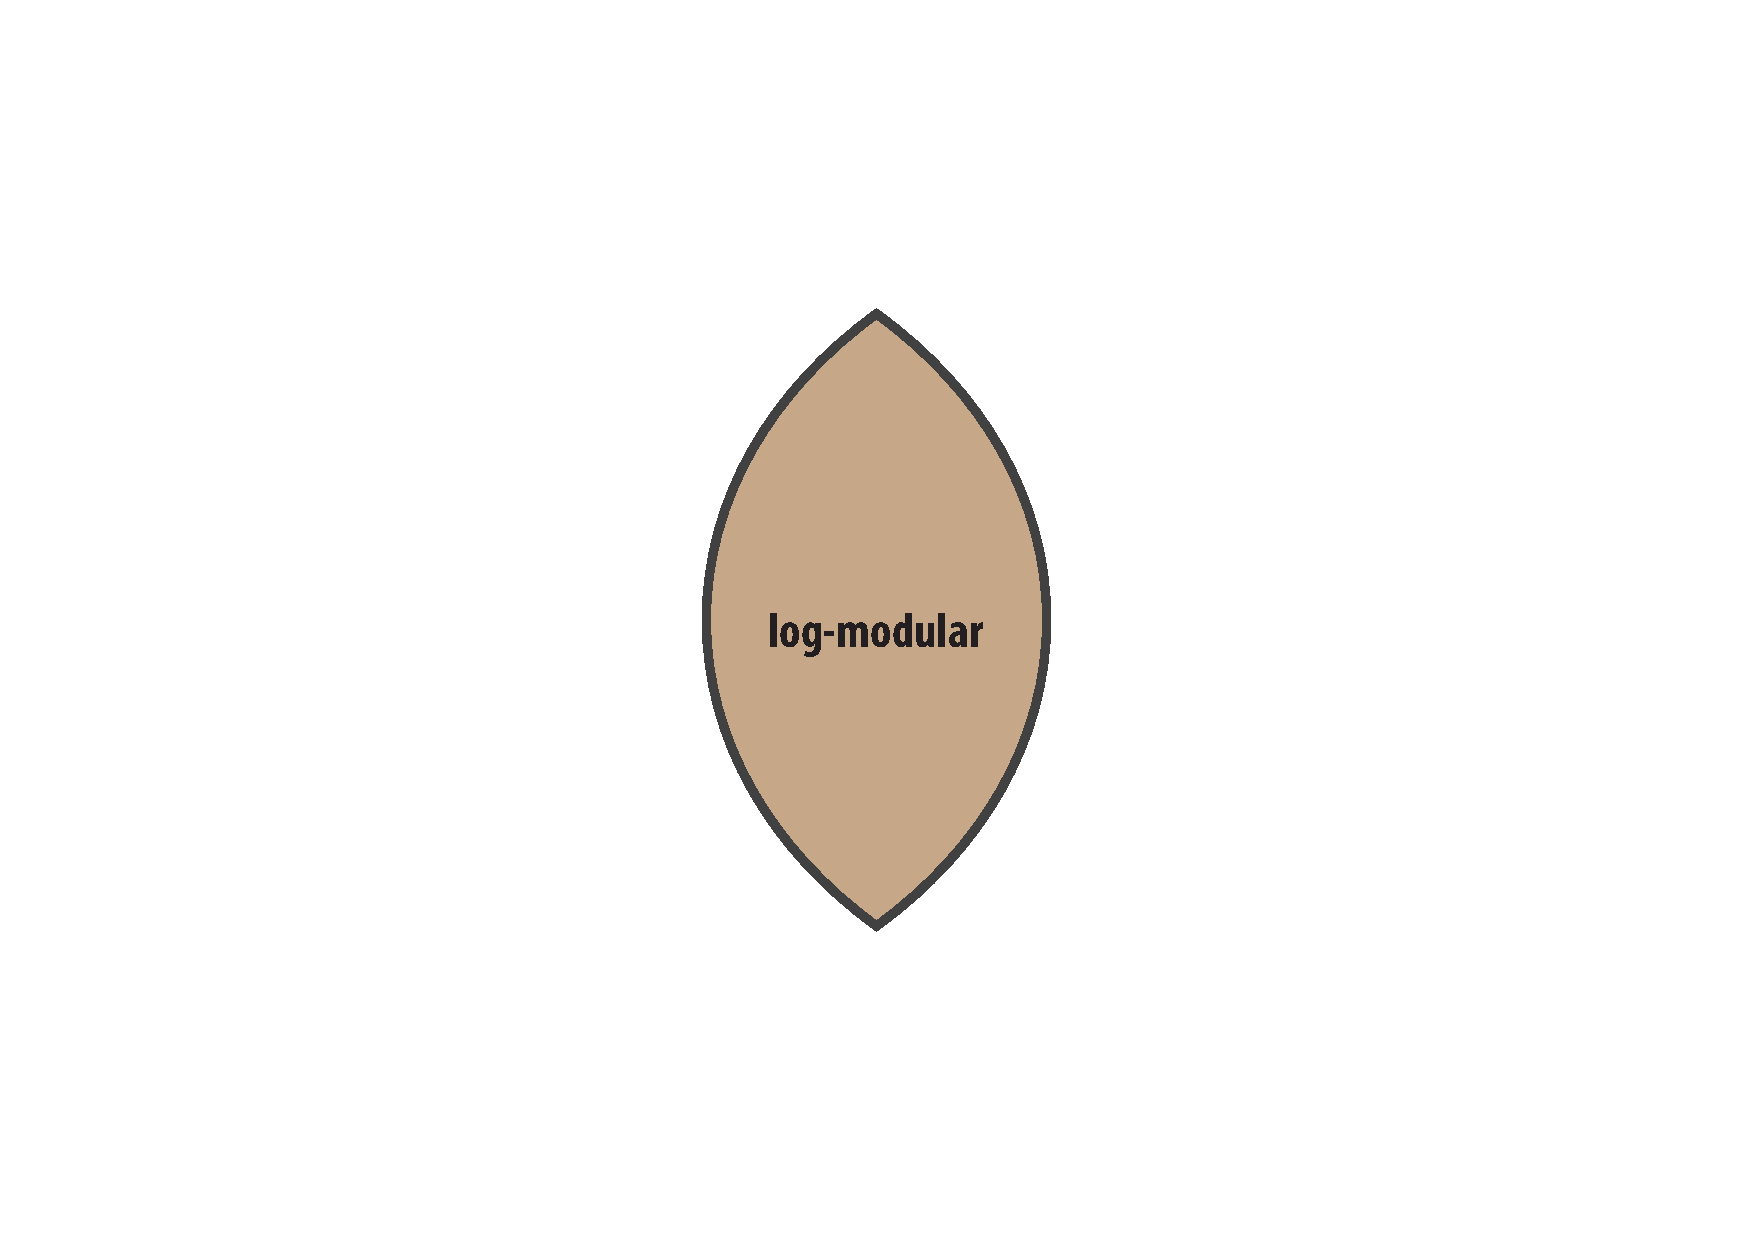
\includegraphics[width=4.3in]{figures/venn01.pdf}}%
\only<2>{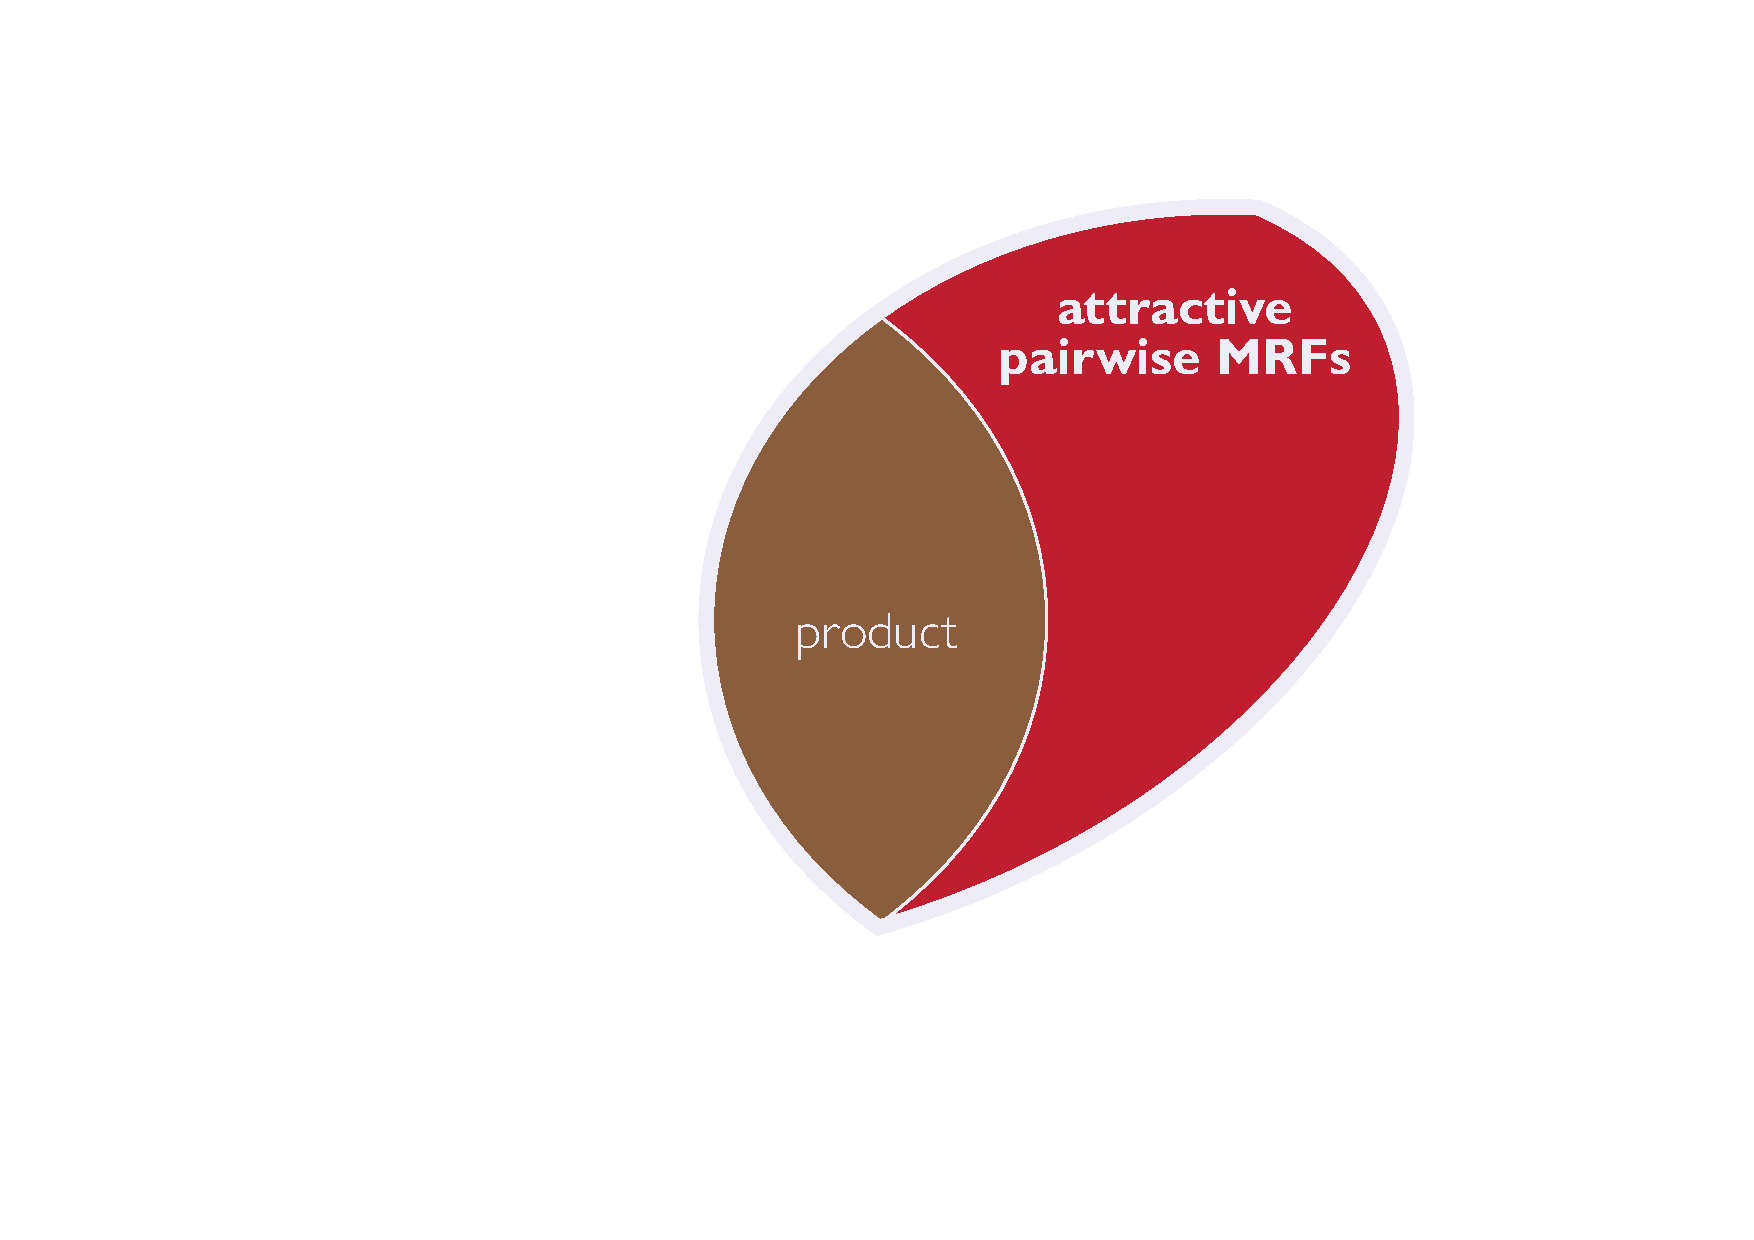
\includegraphics[width=4.3in]{figures/venn02.pdf}}%
\only<3>{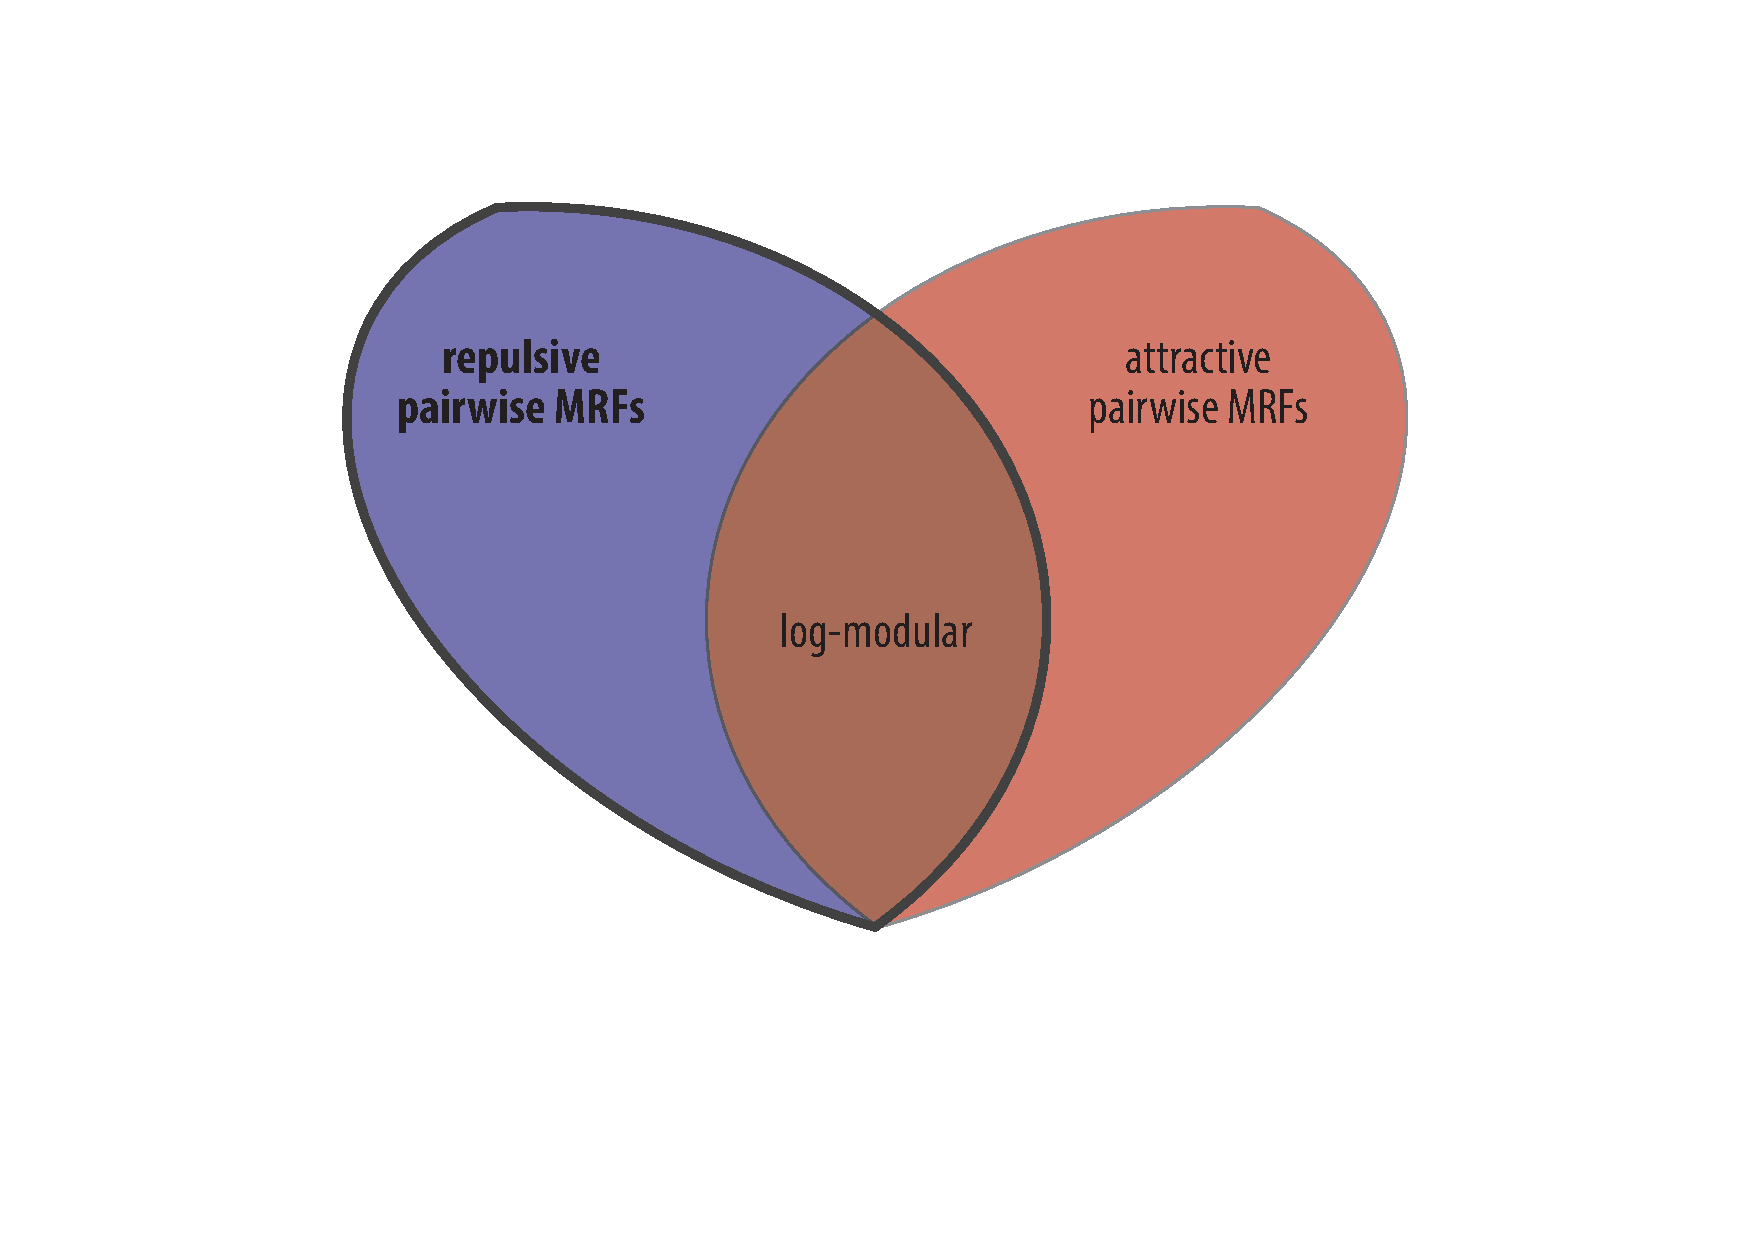
\includegraphics[width=4.3in]{figures/venn03.pdf}}%
\only<4>{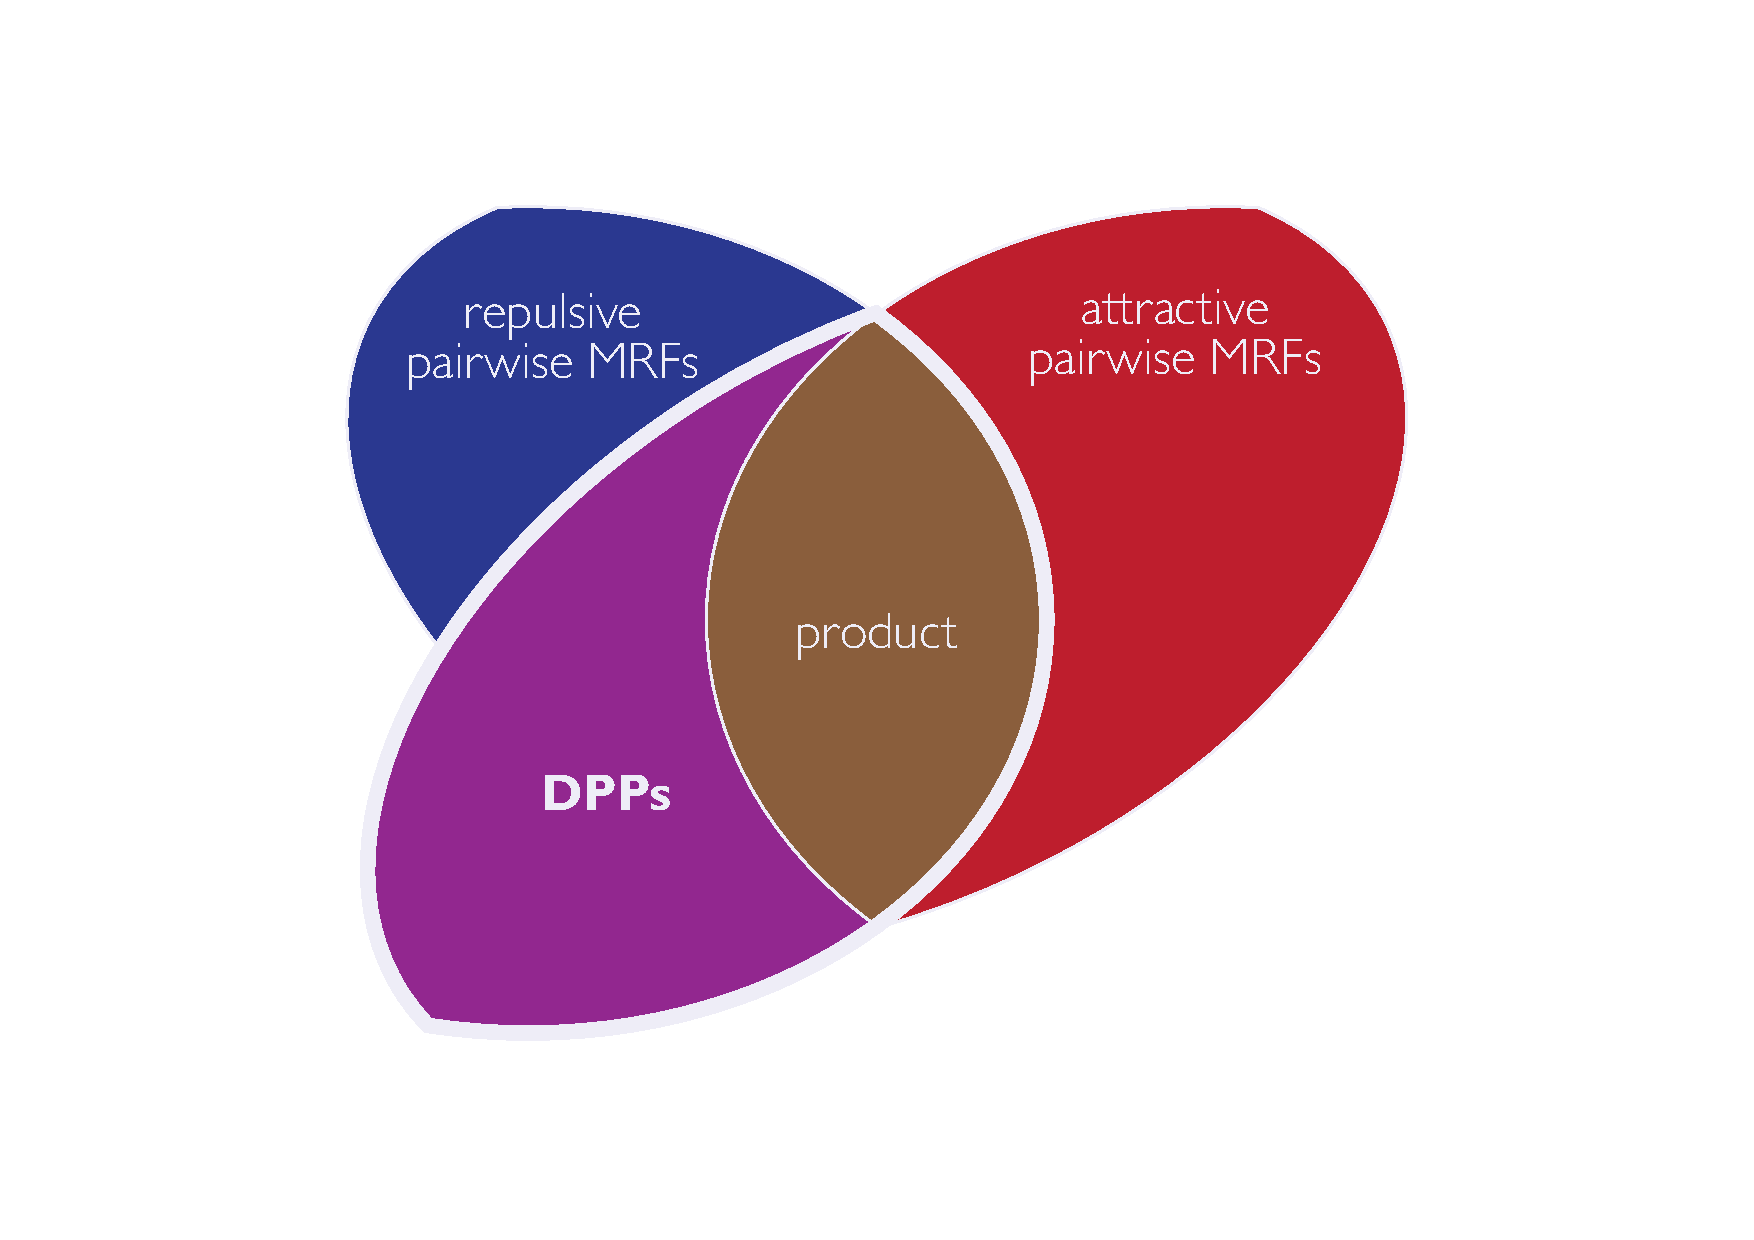
\includegraphics[width=4.3in]{figures/venn04.pdf}}%
\only<5>{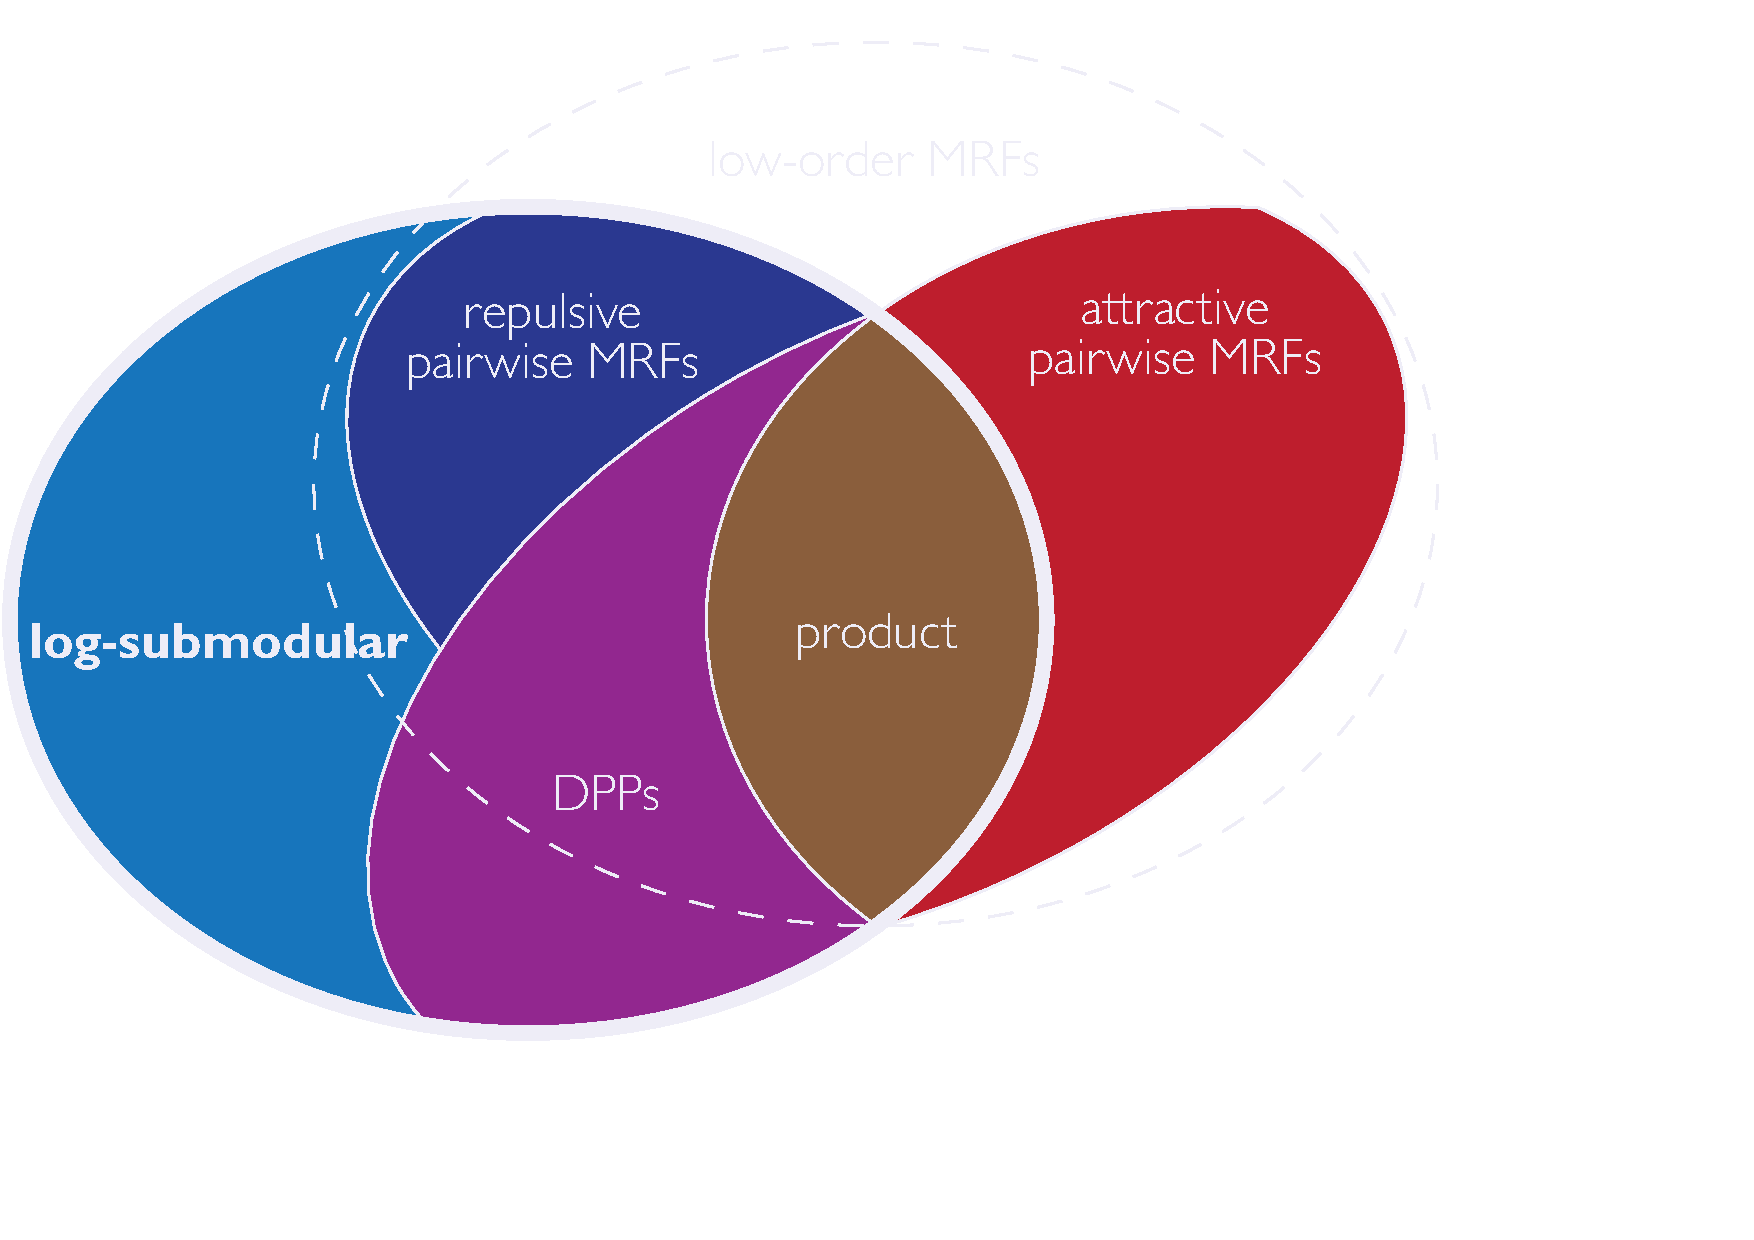
\includegraphics[width=4.3in]{figures/venn06.pdf}}%
\only<6>{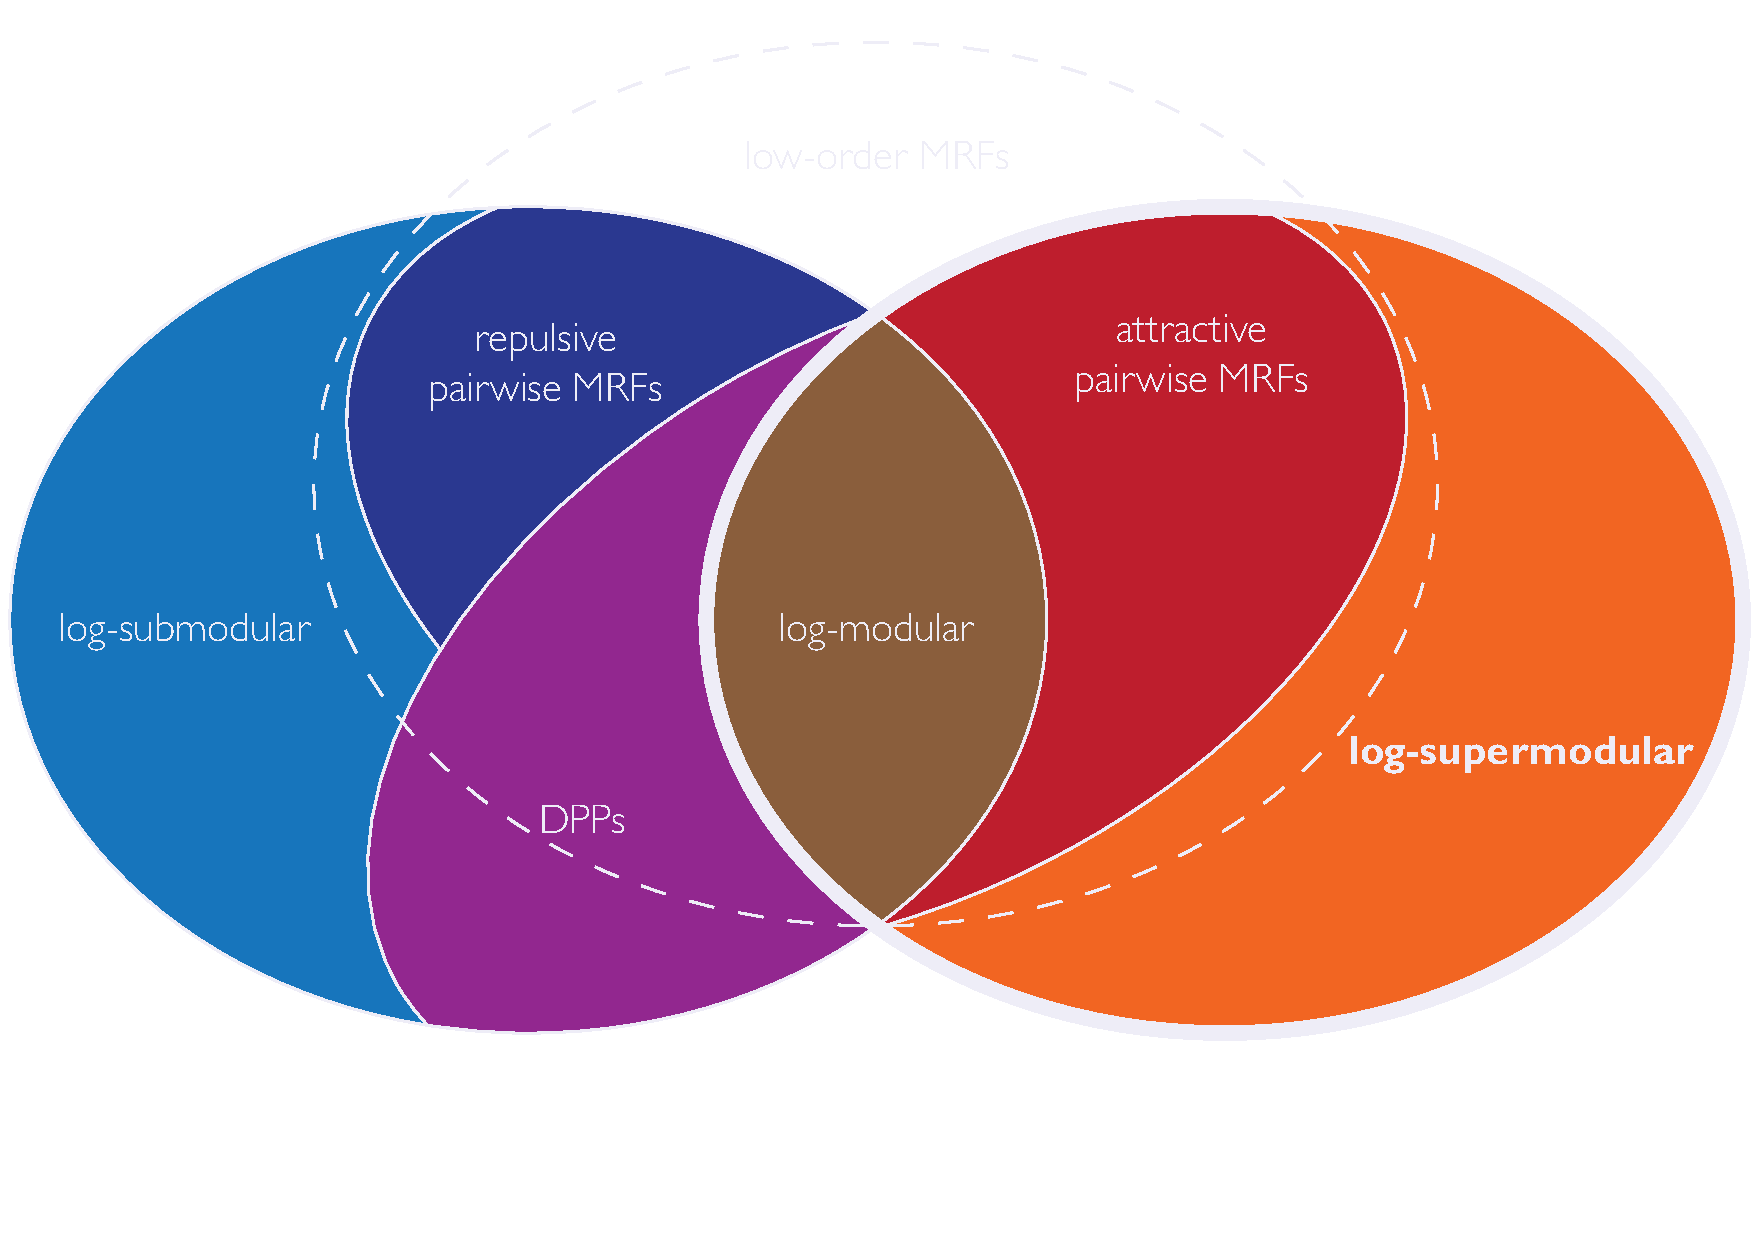
\includegraphics[width=4.3in]{figures/venn07.pdf}}%
\only<7>{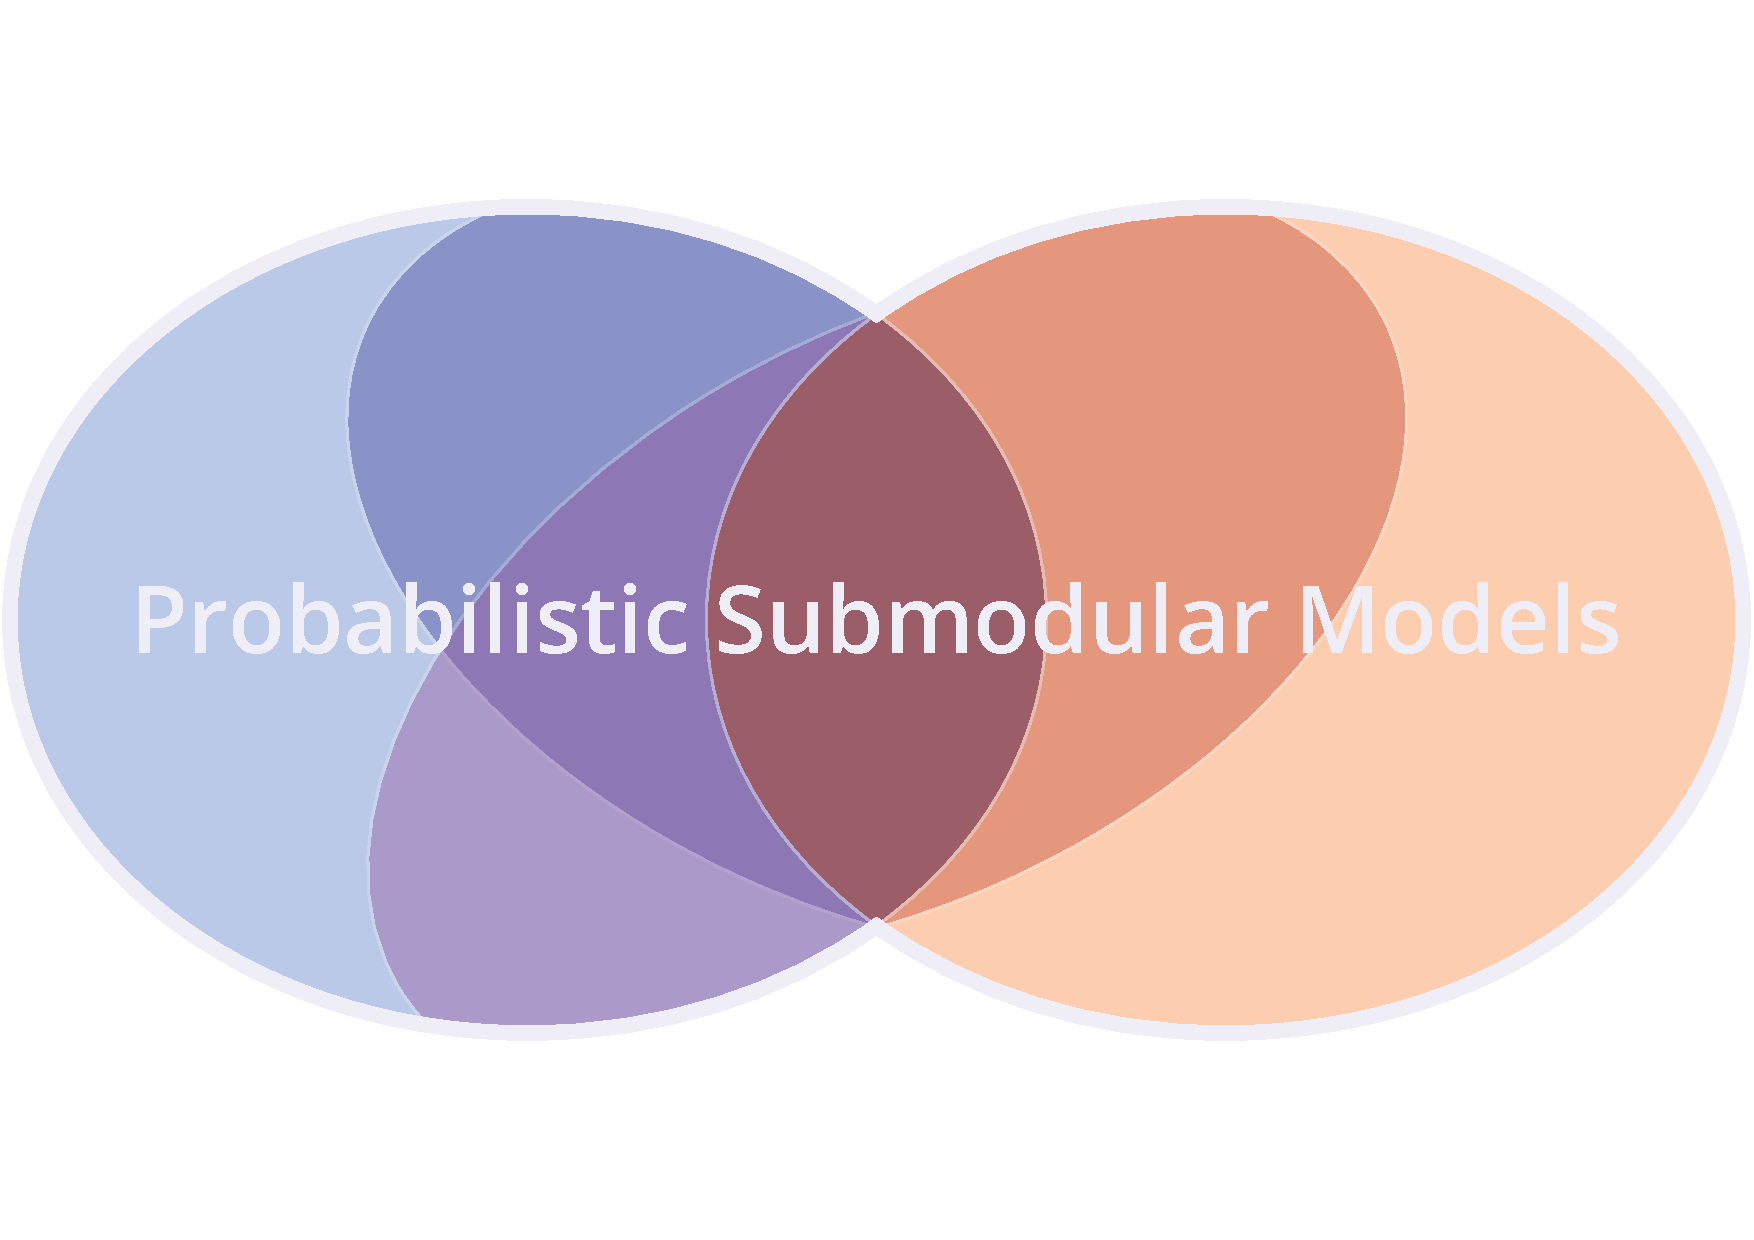
\includegraphics[width=4.3in]{figures/venn08.pdf}}
\end{frame}

\begin{frame}{Inference}
\vspace{1em}
\begin{columns}[c]
\column{0.46\textwidth}
\centering
$\mathbb{P}(\textrm{pixel label})$

\vspace{0.7em}
\centering
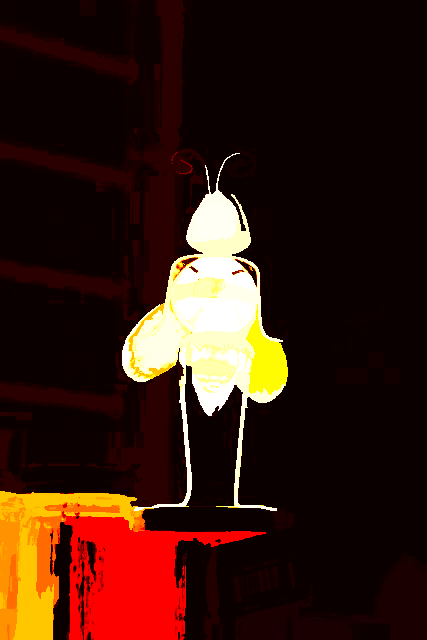
\includegraphics[height=2.6in]{figures/bee_marginals.png}

\column{0.54\textwidth}
\centering
$\mathbb{P}(\textrm{image} \in \textrm{summary} \mid \textrm{selected})$

\vspace{0.7em}
\centering
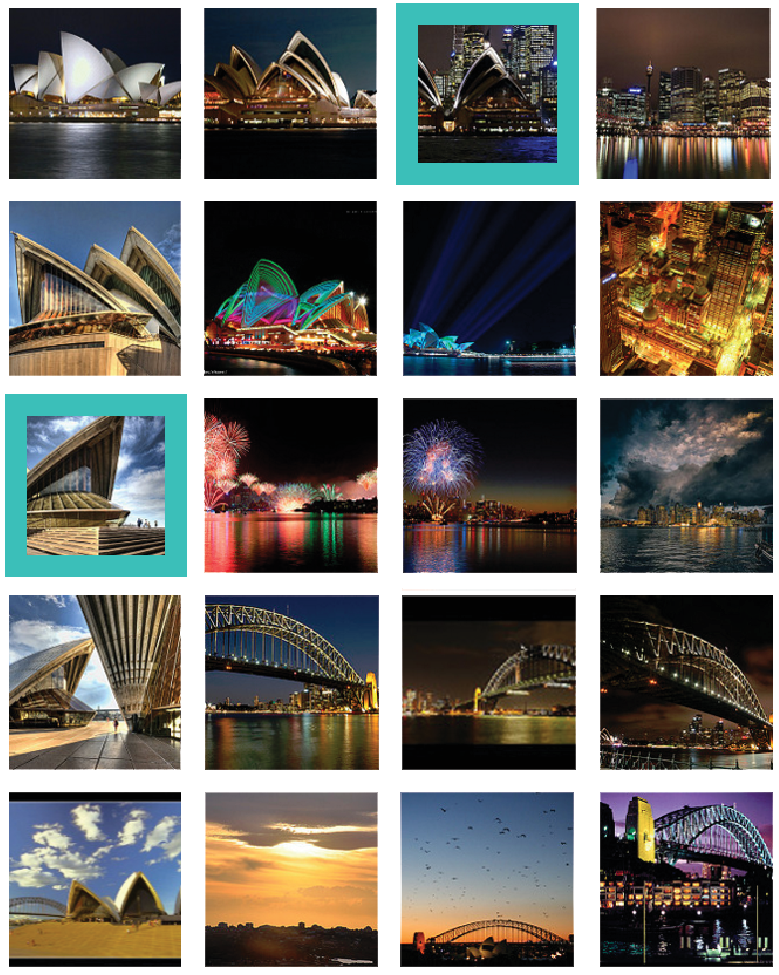
\includegraphics[height=2.6in]{figures/flickr_inference.pdf}
\end{columns}
\end{frame}

\begin{frame}{Inference}
\vspace{1em}

\begin{minipage}{\textwidth}
\begin{columns}[c]
\column{0.43\textwidth}
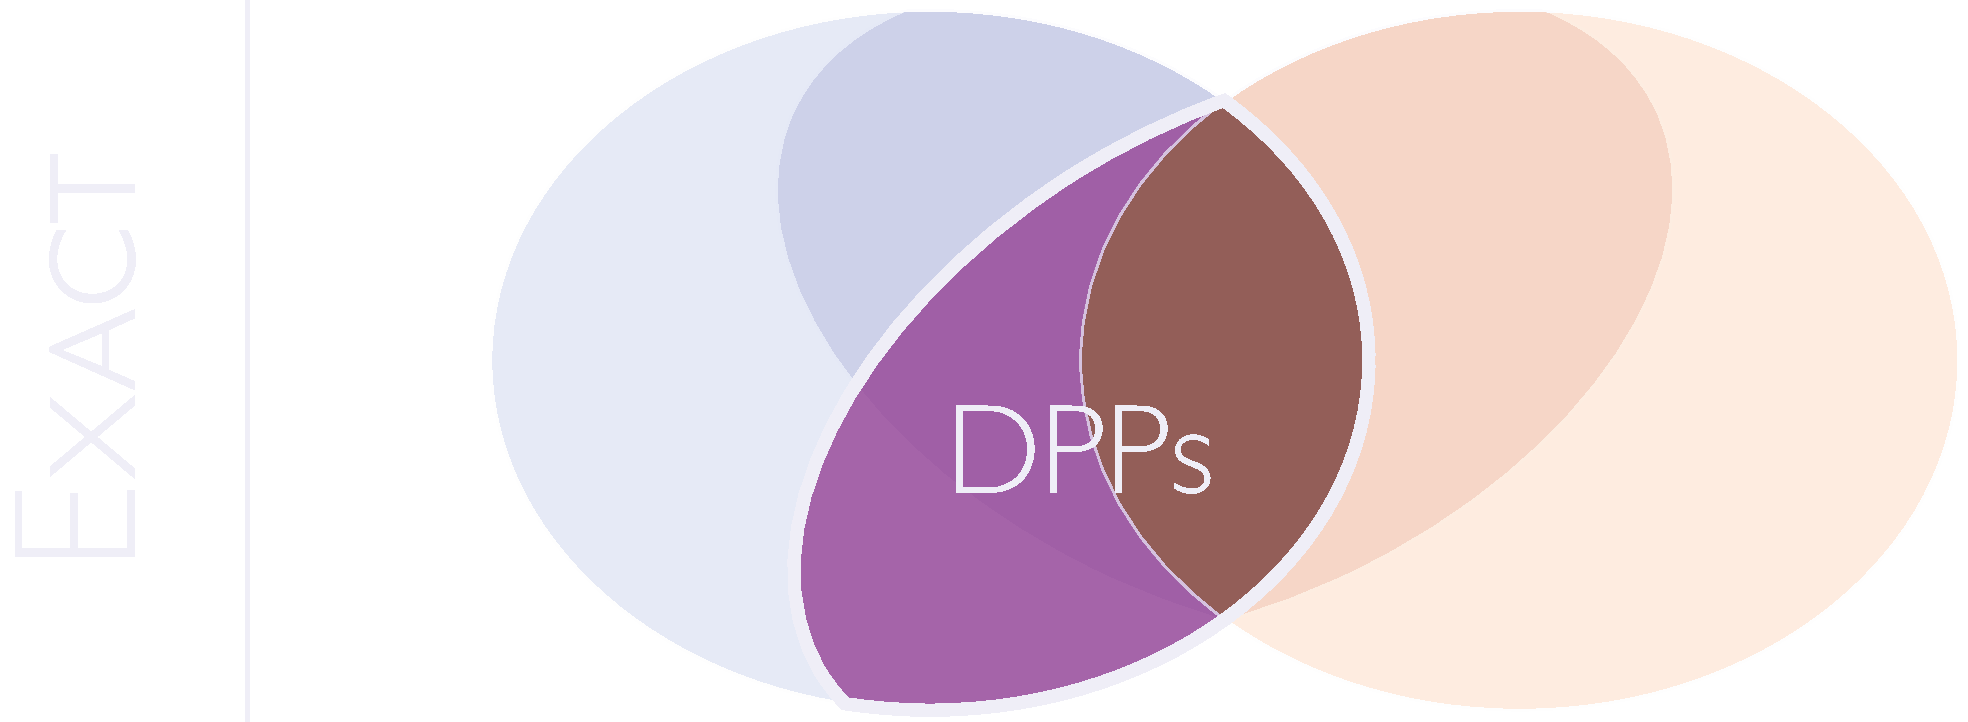
\includegraphics[width=1.85in]{figures/inf01_exact_horz.pdf}
\column{0.57\textwidth}
\begin{itemize}
\item \small{Tractable only for limited subclasses}
\vspace{1em}
\item \small{\#P-hard even for Ising models}
\end{itemize}
\end{columns}
\end{minipage}

\uncover<2->{
\vspace{2em}
\begin{minipage}{\textwidth}
\begin{columns}[c]
\column{0.43\textwidth}
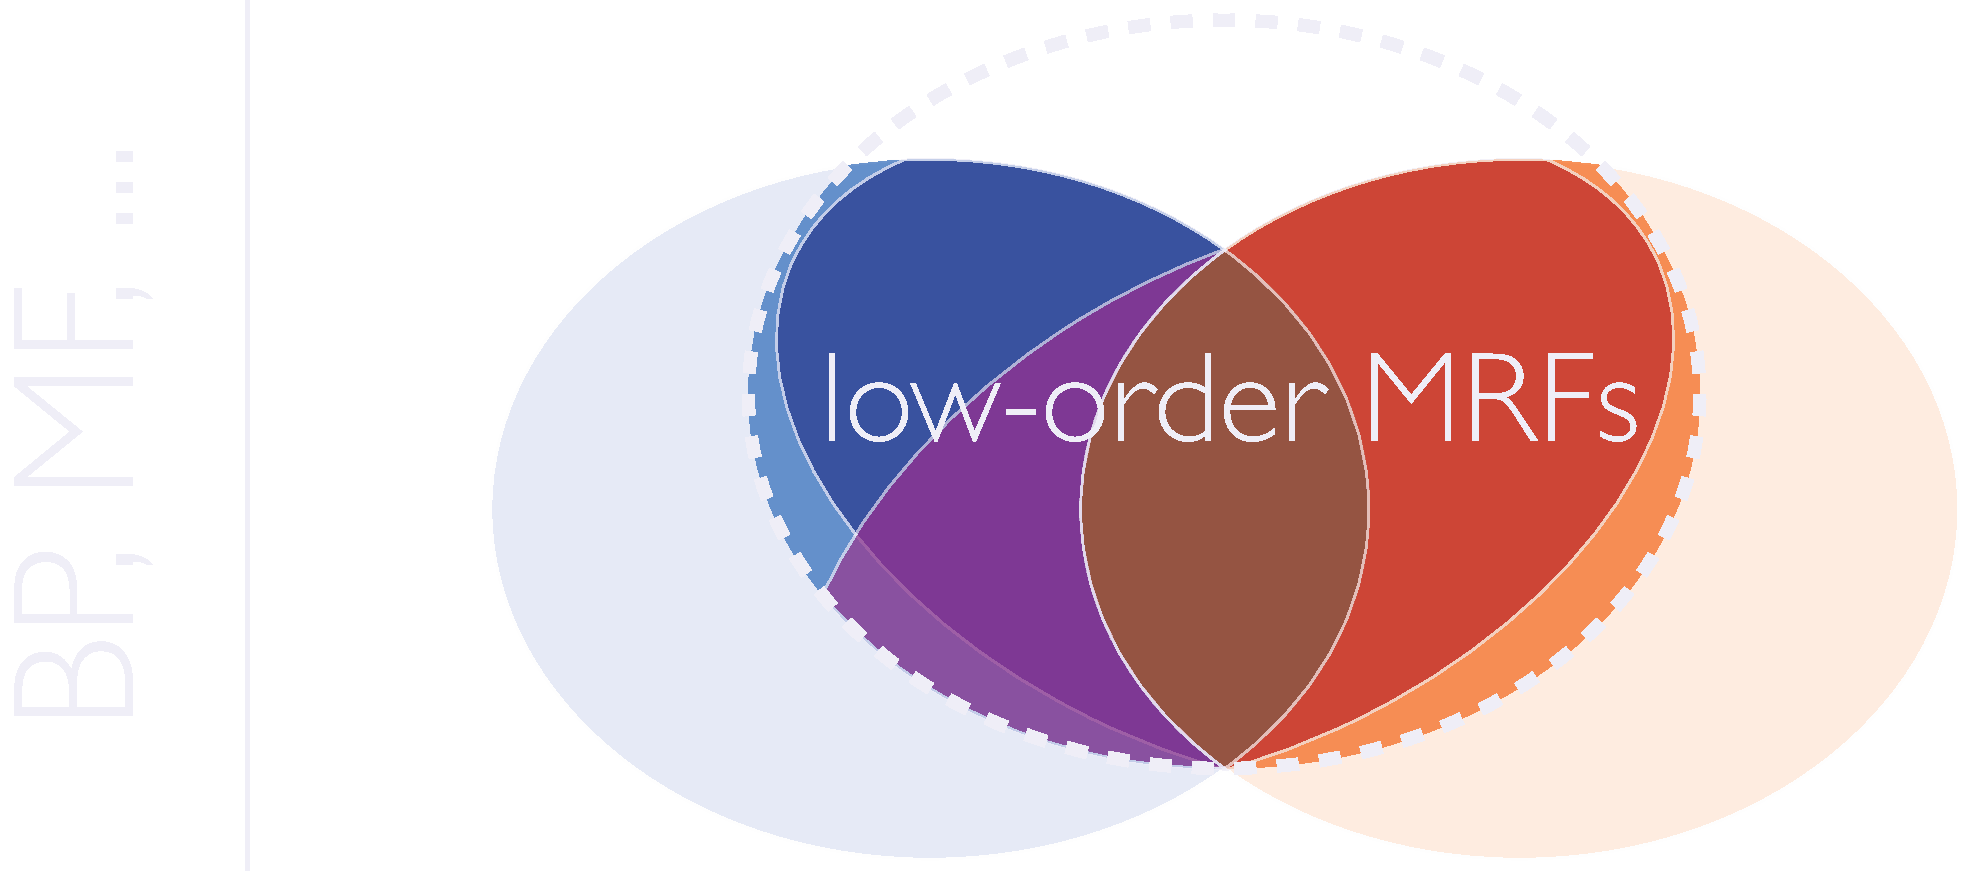
\includegraphics[width=1.85in]{figures/inf02_loworder_horz.pdf}
\column{0.57\textwidth}
\begin{itemize}
\item \small{Extensively studied model class}
\vspace{1em}
\item \small{Complexity exponential in model order}
\end{itemize}
\end{columns}
\end{minipage}
}

\uncover<3->{
\vspace{2em}
\begin{minipage}{\textwidth}
\begin{columns}[c]
\column{0.43\textwidth}
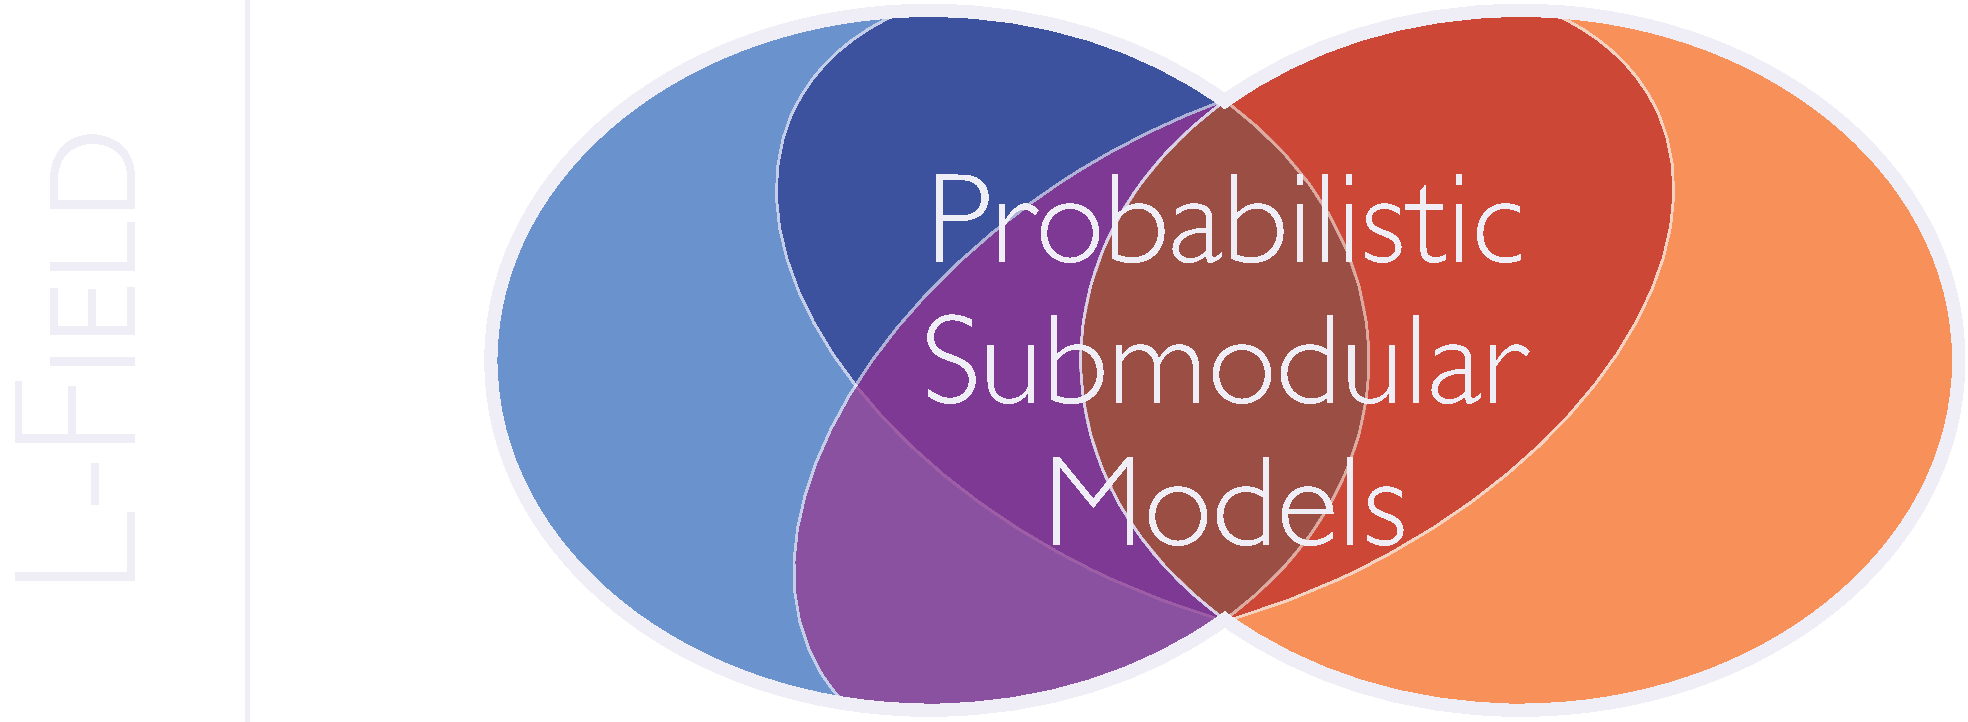
\includegraphics[width=1.85in]{figures/inf03_psm_horz.pdf}
\column{0.57\textwidth}
\begin{itemize}
\item \small{Variational approach for general PSMs} \qcite{Djolonga and Krause, '14}
\end{itemize}
\end{columns}
\end{minipage}
}
\end{frame}

\begin{frame}{Inference}

\centering
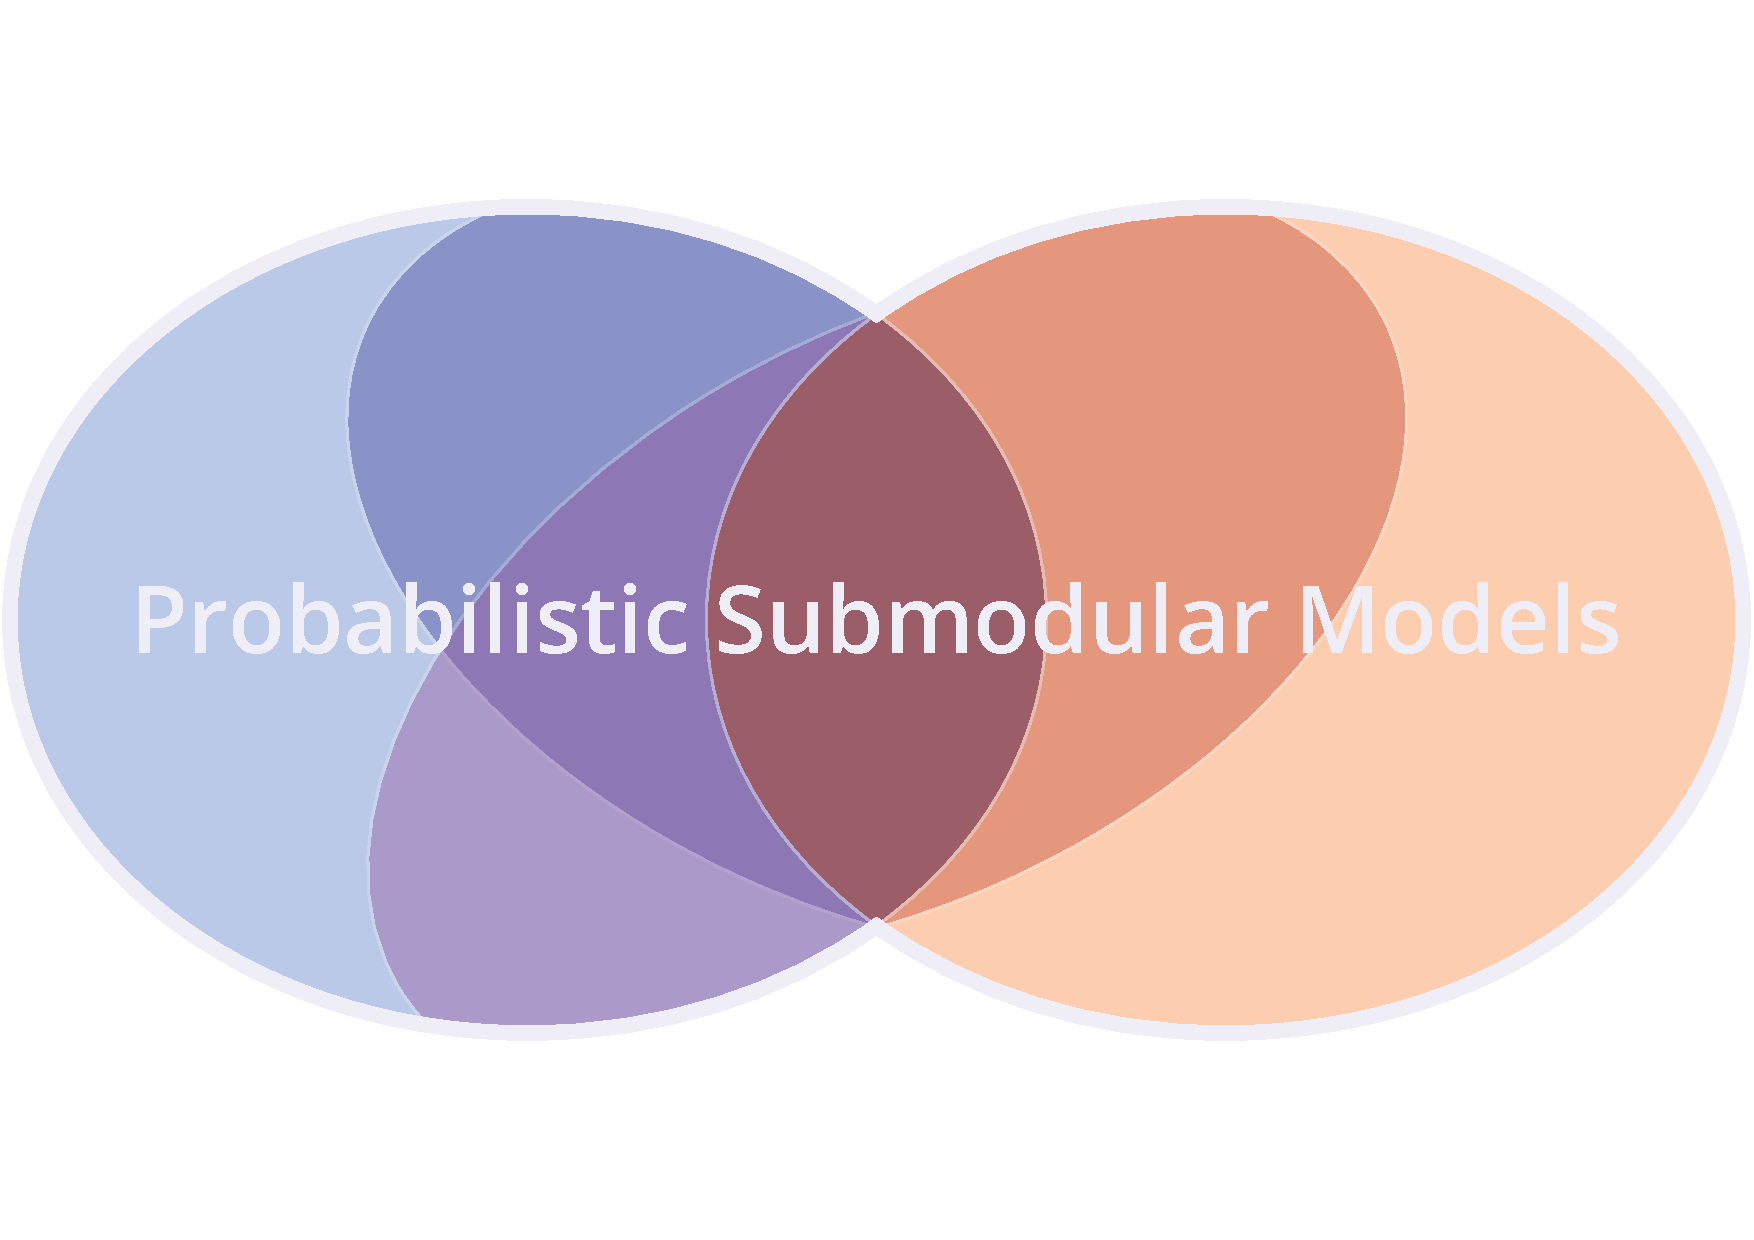
\includegraphics[width=2.5in]{figures/venn08.pdf}

\vspace{0.5em}
\centering
\qboxa{\large \strut What about sampling?}

\end{frame}

\begin{frame}{Markov Chain Monte Carlo}
\begin{tabular}{*{2}{@{}l}}
\begin{minipage}{0.45\textwidth}
\begin{itemize}
\item<1-> State space $\Omega$
\end{itemize}
\end{minipage} & \uncover<3->{\color{col1}powerset of $V$}\\[1.5em]
\begin{minipage}{0.45\textwidth}
\begin{itemize}
\item Transition matrix $P$
\end{itemize}
\end{minipage} & \uncover<4->{\color{col1}Gibbs sampler}\\[1.5em]
\begin{minipage}{0.45\textwidth}
\begin{itemize}
\item Stationary distribution $\pi$
\end{itemize}
\end{minipage} & \uncover<5->{\color{col1}PSM distribution}
\end{tabular}

\uncover<2->{
\vspace{3em}
Markov chain $\left(S_t\right)_{t \geq 0}$ that moves according to $P$
}
\end{frame}

\begin{frame}{State Space of $V = \{1, 2, 3\}$}
\vspace{1em}
\centering
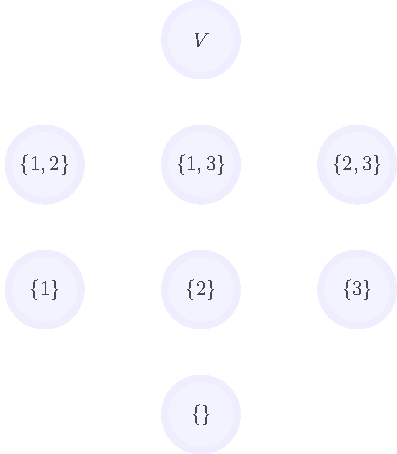
\includegraphics[height=2.7in]{figures/lattice_nodes_only.pdf}
\end{frame}

\begin{frame}{Gibbs Sampler}
\vspace{1em}
\begin{columns}[c]
\column{0.5\textwidth}
\uncover<2->{Start at $S_0$

\vspace{1.1em}
For $t = 1, 2, \ldots$}
\vspace{1.1em}
\begin{itemize}
\item<4-> Select random $v \in V$
\vspace{1.1em}
\item<7-> Compute conditional $p_{\textrm{add}}$
\vspace{1.1em}
\item<8-> Flip biased coin

\vspace{-1em}
\begin{minipage}{0.5\textwidth}\vspace{2em}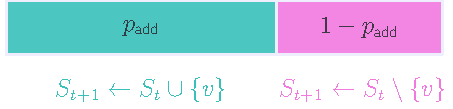
\includegraphics[width=2.5in]{figures/gibbs.pdf}\end{minipage}
\end{itemize}
\column{0.5\textwidth}
\only<1-2>{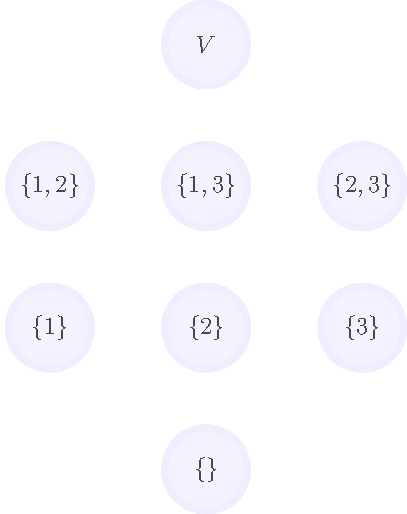
\includegraphics[height=2.5in]{figures/lattice_nodes_only_large.pdf}}%
\only<3-4>{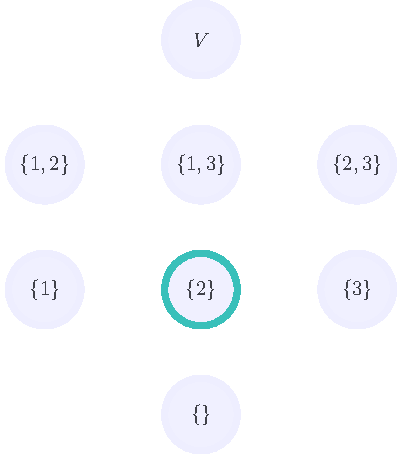
\includegraphics[height=2.5in]{figures/lattice_example_node.pdf}}%
\only<5>{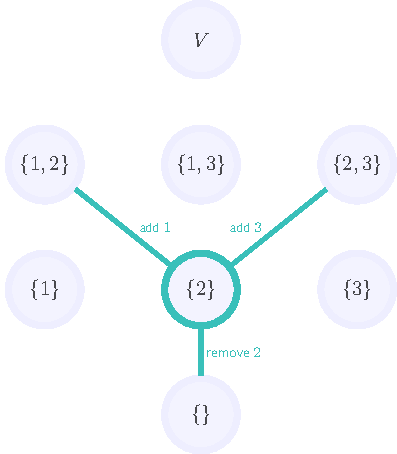
\includegraphics[height=2.5in]{figures/lattice_example_edges.pdf}}%
\only<6-8>{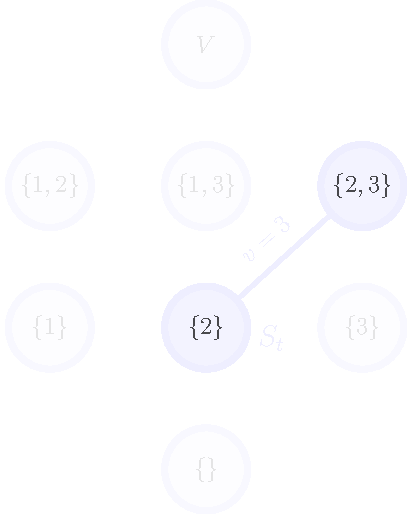
\includegraphics[height=2.5in]{figures/lattice_example_edges_one.pdf}}%
\only<9>{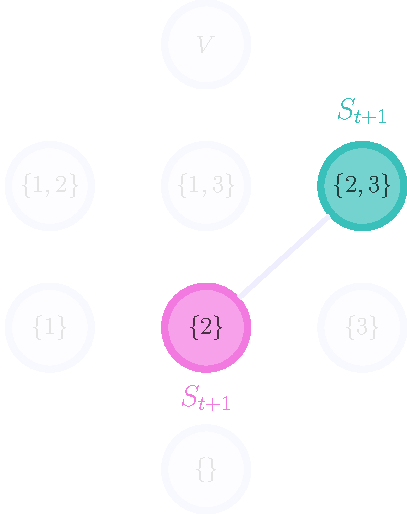
\includegraphics[height=2.5in]{figures/lattice_example_edges_one_trans.pdf}}
\vspace{2em}
\end{columns}
\end{frame}

\begin{frame}{Gibbs Sampler}
\vspace{1em}
\centering
\only<1>{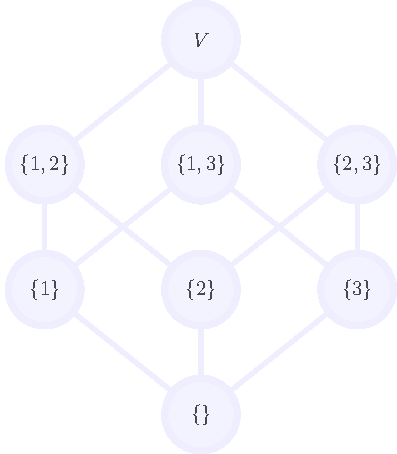
\includegraphics[height=2.7in]{figures/lattice_full.pdf}}%
\only<2>{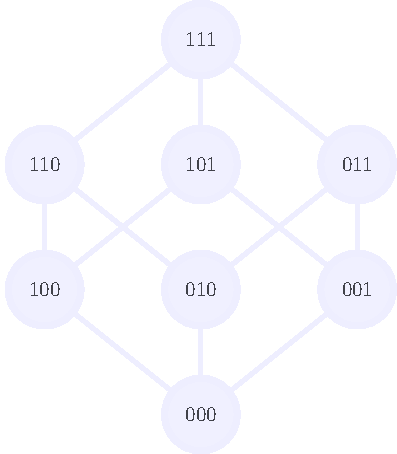
\includegraphics[height=2.7in]{figures/lattice_full_binary.pdf}}
\end{frame}

\begin{frame}{Mixing time}
\vspace{0.5em}
\qboxa{Does the Markov chain converge?}

\vspace{0.5em}
\only<2->{Total variation distance}
\only<2>{
\begin{align*}
d(t) = d_{\mathrm{tv}}\left(\mathbb{P}_{S_t}, \pi\right)
\end{align*}}
\only<3>{
\begin{align*}
d(t) = {\color{col1}\max \{}d_{\mathrm{tv}}\left(\mathbb{P}_{S_t}, \pi\right) {\color{col1}\mid S_0 \in \Omega\}}
\end{align*}
}
\alt<1,4->{\uncover<4->{
\begin{align*}
d(t) = \max \{d_{\mathrm{tv}}\left(\mathbb{P}_{S_t}, \pi\right) \mid S_0 \in \Omega\}
\end{align*}
}}{}

\uncover<4->{
\vspace{-1em}
Under mild assumptions (ergodicity), $\ \ d(t) \xrightarrow{\ t\,\rightarrow\,\infty\ } 0$
}

\uncover<5->{
\vspace{2.5em}
\qboxa{How long does it take to get ``close enough" to $\pi$?}
}

\uncover<6->{
\vspace{1em}
Mixing time $\ \ \ t_{\textrm{mix}}(\epsilon) = \min \left\{t \mid d(t) \leq \epsilon \right\}$
}
\end{frame}

\begin{frame}{Goal}
\begin{itemize}
\item<1-> Mixing times for general PSMs are exponential in $|V| = n$
\vspace{1em}
\item<2-> Exponential even for pairwise models \qcite{Jerrum and Sinclair, '93}
\end{itemize}

\uncover<3->{
\vspace{3em}
\centering
\qboxa{\minibox{We establish sufficient conditions for sub-exponential mixing\\of the Gibbs sampler on PSMs.}}
}
\end{frame}

\begin{frame}{Polynomial-time Mixing}
\vspace{0.5em}
\only<1>{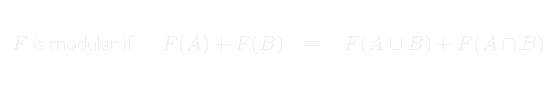
\includegraphics[width=3.9in,trim=5 0 0 0,clip]{figures/ineq_mod_0.pdf}}%
\only<2>{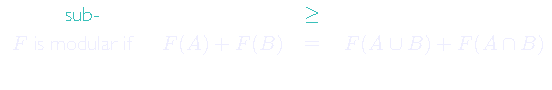
\includegraphics[width=3.9in,trim=5 0 0 0,clip]{figures/ineq_mod_1.pdf}}%
\only<3->{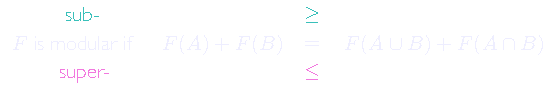
\includegraphics[width=3.9in,trim=5 0 0 0,clip]{figures/ineq_mod_2.pdf}}

\uncover<4->{
\vspace{4em}
``Distance" from modularity
\begin{align*}
\uncover<5->{\zeta_F \coloneqq \max_{A, B \subseteq V}} \uncover<4->{\big|F(A) + F(B) - F(A \cup B) - F(A \cap B)\big|}
\end{align*}
}
\end{frame}

\begin{frame}{Polynomial-time Mixing}
\vspace{0.5em}
\centering
\only<1>{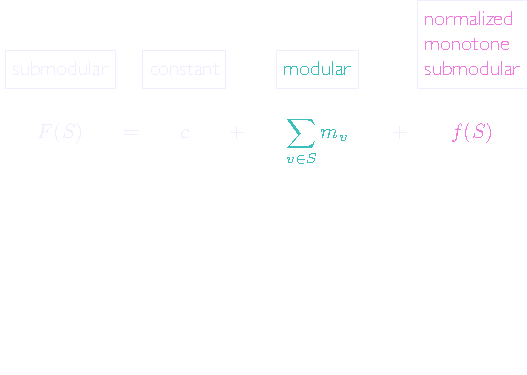
\includegraphics[width=3.9in]{figures/decomp_0.pdf}}%
\only<2>{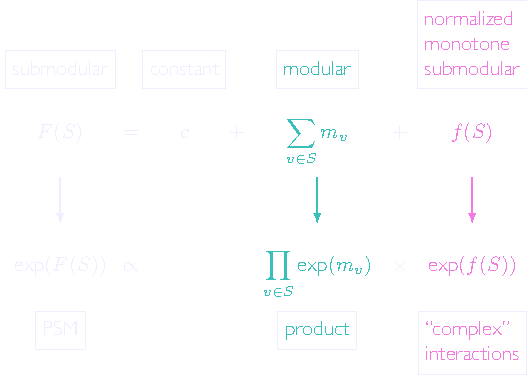
\includegraphics[width=3.9in]{figures/decomp_1.pdf}}
\end{frame}

\begin{frame}{Polynomial-time Mixing}
\qtheorem{1}{
For any submodular or supermodular set function $F$, the mixing time of the Gibbs sampler is bounded by
\begin{align*}
t_{\textrm{mix}}(\epsilon) = \mathcal{O}\left(n^2 \exp(\zeta_f)\log\epsilon^{-1}\right).
\end{align*}
}
\end{frame}

\begin{frame}{Polynomial-time Mixing}
\vspace{0.5em}
\begin{columns}[c]
\column{0.5\textwidth}
\centering
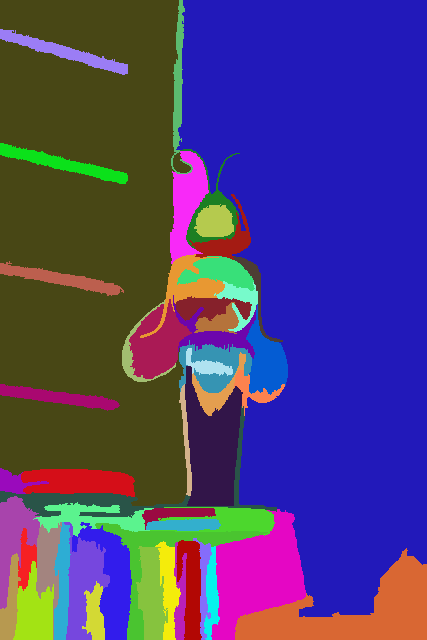
\includegraphics[width=1.8in]{figures/bee_superpixels.png}
\column{0.5\textwidth}
$F_i(S) = \phi\left(|S \cap V_i|\right)$

\vspace{1em}
$F(S) = \displaystyle\sum_{i=1}^L F_i(S)$

\uncover<2->{
\vspace{3em}
Easy to show that

\vspace{0.5em}
\hspace{2em}$\zeta_f \leq L \phi_{\textrm{max}}$
}

\uncover<3->{
\vspace{3em}
\qboxa{
$|V_i| \approx 10^5\ $ vs. $\ L \approx 50$
}
}
\end{columns}
\end{frame}

\begin{frame}{Proof Outline}
\vspace{1em}
\only<1>{Method of canonical paths \qcite{Sinclair, '92}}%
\only<2>{For each $A, B \subseteq V$, need to route $p(A)p(B)$ amount of flow}%
\only<3-7>{Construct a ``canonical path'' between each $A, B \subseteq V$}%
\only<8>{Capacity of an edge $\ \sim\ $ transition probability of Gibbs sampler}%
\only<9>{Congestion of an edge $\ \sim\ $ (total flow through edge) / capacity}%
\only<10>{$t_{\mathrm{mix}}(\epsilon) = \mathcal{O}\left(\max\{\textrm{congestion}\}\log \epsilon^{-1}\right)$ \qcite{Sinclair, '92}}%
\only<11>{We bound the maximum congestion of a PSM using $\zeta_f$}

\vspace{1em}
\centering
\only<1>{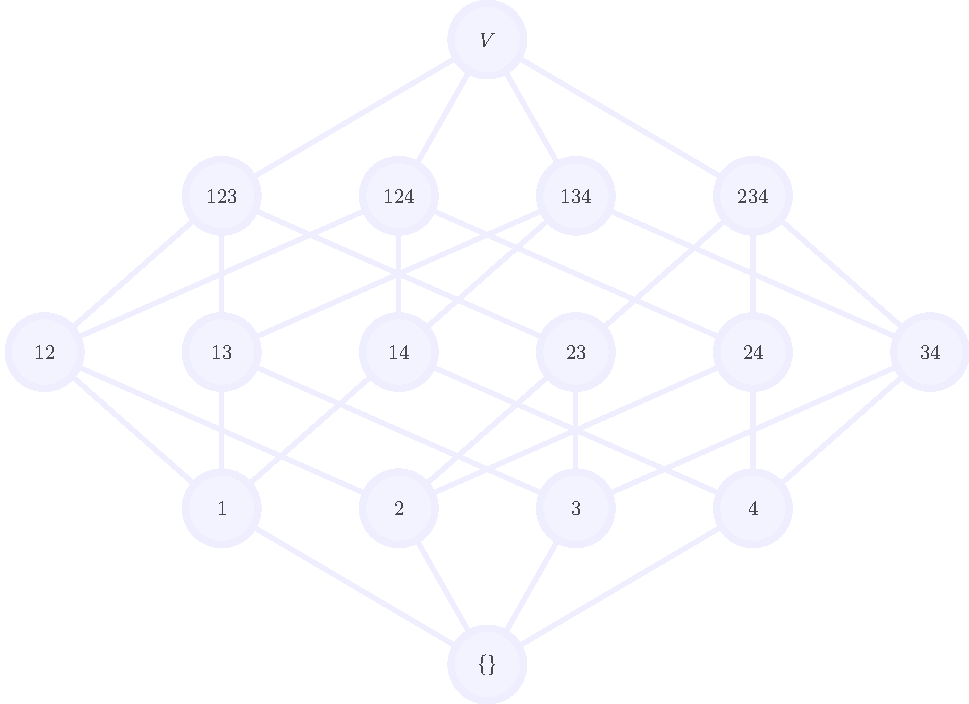
\includegraphics[width=3.6in]{figures/cp_intro.pdf}}%
\only<2>{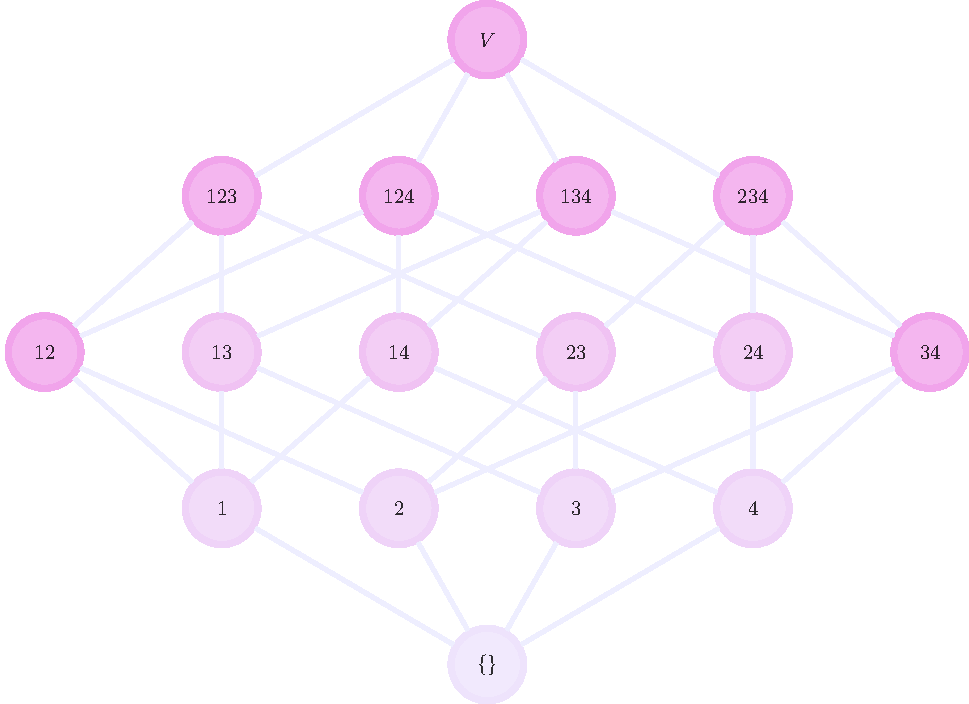
\includegraphics[width=3.6in]{figures/cp_easy_nodes_only.pdf}}%
\only<3>{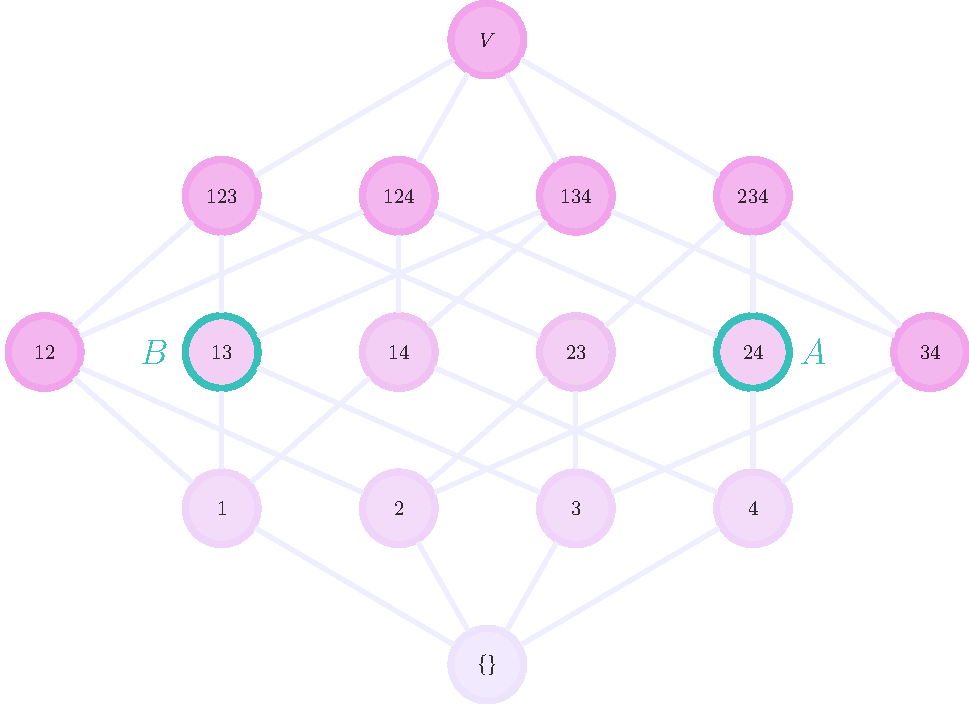
\includegraphics[width=3.6in]{figures/cp_easy_path_0.pdf}}%
\only<4>{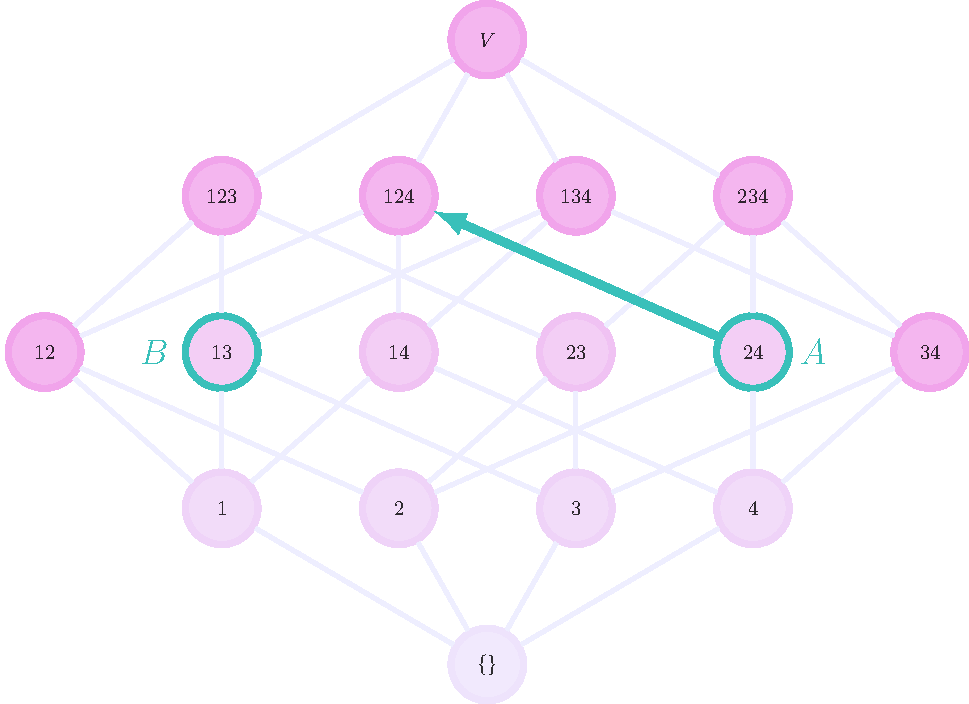
\includegraphics[width=3.6in]{figures/cp_easy_path_1.pdf}}%
\only<5>{\includegraphics[width=3.6in]{figures/cp_easy_path_2.pdf}}%
\only<6>{\includegraphics[width=3.6in]{figures/cp_easy_path_3.pdf}}%
\only<7>{\includegraphics[width=3.6in]{figures/cp_easy_path_4.pdf}}%
\only<8>{\includegraphics[width=3.6in]{figures/cp_easy.pdf}}%
\only<9-11>{\includegraphics[width=3.6in]{figures/cp_easy_cong.pdf}}
\end{frame}

\begin{frame}{Fast Mixing}
\vspace{0.5em}
\qtheorem{2}{
For any submodular or supermodular set function $F$, if $\gamma_f < 1$, the mixing time of the Gibbs sampler is bounded by
\vspace{-0.5em}
\begin{align*}
t_{\textrm{mix}}(\epsilon) \leq \frac{1}{1 - \gamma_f} n \left(\log n + \log\epsilon^{-1}\right).
\end{align*}
}

\vspace{0.5em}
\begin{itemize}
\item<1-> $\gamma_f$ = ``maximum total influence''
\vspace{0.5em}
\item<2-> Simple way to bound $\gamma_f$, if $f(S) = \sum_i f_i(S)$
\vspace{0.5em}
\item<3-> Closely related to Dobrushin uniqueness conditions, and influence matrix norms \qcite{Dyer et al., '09}
\vspace{0.5em}
\item<4-> Similar theorem by \qcite{Rebeschini and Karbasi, '15}
\end{itemize}
\end{frame}

\begin{frame}{Evaluation}
\vspace{0.5em}

Compare against variational approach \qcite{Djolonga and Krause, '14}

\vspace{2em}
\centering
\only<1>{\includegraphics[width=3.5in,clip]{figures/experiments_0.pdf}}%
\only<2->{\includegraphics[width=3.5in,clip]{figures/experiments_1.pdf}}

\vspace{2em}
\begin{itemize}
\item<3-> Compute $\ p(v \mid S)$
\vspace{0.5em}
\item<4-> $|V| = 20$ $\ \ \longrightarrow\ \ $ compare to exact marginals
\end{itemize}
\end{frame}

\begin{frame}{Evaluation}
\vspace{1em}
\centering
\only<1>{\includegraphics[width=4.15in,trim=6 0 0 0,clip]{figures/floc_0.pdf}}%
\only<2>{\includegraphics[width=4.15in,trim=6 0 0 0,clip]{figures/floc_1.pdf}}%
\only<3>{\includegraphics[width=4.15in,trim=6 0 0 0,clip]{figures/floc_2.pdf}}%
\only<4>{\includegraphics[width=4.15in,trim=6 0 0 0,clip]{figures/floc_3.pdf}}%
\only<5>{\includegraphics[width=4.15in,trim=6 0 0 0,clip]{figures/floc_4.pdf}}%
\only<6>{\includegraphics[width=4.15in,trim=6 0 0 0,clip]{figures/floc_5.pdf}}
\end{frame}

\begin{frame}{Conclusion}
\begin{columns}[c]
\column{0.5\textwidth}
\centering \uncover<1->{
\includegraphics[width=2in]{figures/venn08.pdf}}
\column{0.5\textwidth}
\centering \uncover<2->{
\includegraphics[height=1.9in]{figures/lattice_full.pdf}}
\end{columns}

\vspace{1em}
\begin{itemize}
\item<3-> Identify higher-order models amenable to efficient inference
\vspace{1em}
\item<4-> First indications that sub-/supermodularity can lead to faster mixing
\end{itemize}

\uncover<5->{
\vspace{1em}
\centering
\qboxa{Poster \#70}
}
\end{frame}

\begin{frame}{Backup I}
\vspace{1em}
Start at $S_0$

\vspace{1.1em}
For $t = 1, 2, \ldots$
\vspace{1.1em}
\begin{itemize}
\item Select random $v \in V$
\vspace{1.1em}
\item $\Delta \gets F(S_t \cup \{v\}) - F(S_t \setminus \{v\})$
\vspace{1.1em}
\item $p_{\textrm{add}} \gets e^{\Delta} / \left(1 + e^{\Delta}\right)$
\vspace{1.1em}
\item Flip biased coin

\vspace{-1em}
\begin{minipage}{0.5\textwidth}\vspace{2em}\includegraphics[width=2.5in]{figures/gibbs.pdf}\end{minipage}
\end{itemize}
\end{frame}

\begin{frame}{Backup II}
\vspace{0.5em}
\centering
\includegraphics[width=4.3in]{figures/venn07_old_nobold.pdf}
\end{frame}

\begin{frame}{Backup III}
\qtheorem{1}{
For any set function $F$, the mixing time of the Gibbs sampler is bounded by
\begin{align*}
t_{\textrm{mix}}(\epsilon) = \mathcal{O}\left(n^2 \exp({\color{col1}2\zeta_F})\log\epsilon^{-1}\right).
\end{align*}

\vspace{1em}
For any {\color{col1}submodular or supermodular} set function $F$, the mixing time of the Gibbs sampler is bounded by
\begin{align*}
t_{\textrm{mix}}(\epsilon) = \mathcal{O}\left(n^2 \exp({\color{col1}\zeta_f})\log\epsilon^{-1}\right).
\end{align*}
}
\end{frame}

\end{document}
